\chapter{运算}
\label{chap:linear-operations}

第~\ref{chap:linear-representation}章把标量、向量、矩阵和映射用基与坐标记录下来。记录本身不回答“怎样算”：两个预测分支的输出怎样合并，两个映射怎样先后作用，一个数组换一种排列后哪些量改变，怎样判断两个方向是否垂直，一个误差向量究竟算多大，一组向量张成的体积有多大，多轴数据又怎样组合与汇总。本章在实数、有限维范围内逐一规定这些基本运算：每种运算说明它做什么、输入输出满足什么条件，以及可以直接使用的性质。第~\ref{chap:sets-functions-and-proofs}章已经给出逐项加减、数乘和行列相乘的算式，这里不重复算术教程。

运算按作用分为三组。第一组把对象合并成同类对象：加法与数乘（\ref{sec:ls-addition-scaling}），逐项乘法、矩阵乘法以及由反复相乘得到的矩阵幂（\ref{sec:ls-multiplication}），还有只改变记录位置的转置与重排（\ref{sec:ls-reshaping}）。第二组给对象以几何：内积把两个对象配成标量并规定垂直（\ref{sec:ls-inner-products}），范数为对象给出大小（\ref{sec:ls-norms-distances}），伴随把内积配对中的作用从一侧搬到另一侧（\ref{sec:ls-adjoints}）。第三组处理多个槽位：外积与行列式测量一组向量张成的有向体积（\ref{sec:ls-exterior-determinants}），张量积、Kronecker积与缩约组织多轴数据的组合与汇总（\ref{sec:ls-tensor-operations}）。

% 第5章：加法与数乘、乘法（逐项乘法、矩阵乘法、矩阵幂）、转置与重排、内积、范数与距离、伴随。

\section{加法与数乘}
\label{sec:ls-addition-scaling}

第~\ref{chap:sets-functions-and-proofs}章已经按对应坐标定义了向量、矩阵的逐项相加与实数数乘，第~\ref{sec:ls-vector-spaces}节又把这些规则抽象为线性空间公理。本节不再重复逐项算式，只回答两个实际问题：两个对象或两个映射在什么条件下可以相加，以及按结构组织计算时实际付出多少。

\subsection{定义与性质}

两个数组能够相加，首先要求形状相同、对应索引的含义相同：$\bm A,\bm B\in\mathbb R^{m\times n}$才有$(\bm A+\bm B)_{i,j}=a_{i,j}+b_{i,j}$，向量$\bm x,\bm y\in\mathbb R^d$才有$(\bm x+\bm y)_j=x_j+y_j$。形状不同的数组不能逐项配对；即使元素总数恰好相同，把$m\times n$与$p\times q$直接相加也没有定义，因为第$(i,j)$个位置在两张表中可能记录不同的量。数乘$c\bm A$把每个元素乘以同一个实数$c$，不改变形状。

逐项规则只用到实数加法与乘法，因此第~\ref{sec:ls-vector-spaces}节列出的交换律、结合律、零元与负元、数乘分配律都按位置各自成立，不需要新的验证。需要单独记住的是相容条件：$\bm A+\bm B$合法当且仅当两者属于同一个同型数组空间。

\paragraph{线性组合与张成}
\label{sec:linear-algebra-map-addition}

若干同型对象分别乘以系数后相加，就是它们的\term{线性组合}：$\sum_{j=1}^k c_j\bm A_j$的每个位置是对应位置元素的同一组合。系数$c_j$是实数，不要求非负，也不要求和为$1$；固定一组系数，线性组合把多个记录合并成一个同型记录。

映射也可以叠加。设$T,S:V\to W$是同一对空间之间的两个线性映射，定义
\[
 (aT+bS)(\bm x)=aT\bm x+bS\bm x,\qquad \bm x\in V,
\]
其中$a,b\in\mathbb R$。叠加保持线性：把输入的线性组合代入，两个分支分别展开再汇总即可。在$V$与$W$的固定基下，$T,S$的矩阵为$\bm A,\bm B$，则$aT+bS$的矩阵就是$a\bm A+b\bm B$。

相加的前提是两个映射的定义域与陪域都一致。这并不要求$V=W$：两个从$\mathbb R^2$到$\mathbb R^3$的映射照样可以相加，只是不能与一个从$\mathbb R^3$到$\mathbb R^2$的映射相加。系数$a,b$必须与输入无关；若叠加系数随$\bm x$改变，叠加后的映射一般不再线性，需要单独检验。

\section{乘法}
\label{sec:ls-multiplication}

“相乘”在线性代数里有两种互不相同的含义。逐项乘法在对应位置把两个同形数组配对相乘，不汇总任何索引；矩阵乘法把两个映射经中间空间复合，对被消去的索引求和。二者输入条件、输出形状和线性性都不同。同一个方阵与自身反复复合得到矩阵幂，它是矩阵乘法的特例，放在本节最后。

\subsection{逐项乘法}

\subsubsection{定义与性质}

\paragraph{逐项乘积（Hadamard积）}

设$\bm A,\bm B\in\mathbb R^{m\times n}$，\term{逐元素乘积}（Hadamard product）记作$\bm A\odot\bm B$，定义为
\begin{equation}
 (\bm A\odot\bm B)_{i,j}=a_{i,j}b_{i,j},
 \label{eq:ls-hadamard}
\end{equation}
输出仍是$m\times n$，每个位置只取两个因子在同一位置的数相乘，不对任何索引求和。例如
\[
 \begin{bmatrix}1&2\\3&4\end{bmatrix}
 \odot
 \begin{bmatrix}0&1\\1&0\end{bmatrix}
 =
 \begin{bmatrix}0&2\\3&0\end{bmatrix}.
\]
它适合表达“用一个掩码挑选或调制另一个数组”：固定掩码$\bm M$后，$\bm X\mapsto\bm M\odot\bm X$把$\bm M$为零的位置置零，把非零位置按系数缩放。

由于等式~\eqref{eq:ls-hadamard} 右端只是实数乘法，按位置逐项验证即得交换律$\bm A\odot\bm B=\bm B\odot\bm A$、结合律$(\bm A\odot\bm B)\odot\bm C=\bm A\odot(\bm B\odot\bm C)$，以及对加法的分配律$\bm A\odot(\bm B+\bm C)=\bm A\odot\bm B+\bm A\odot\bm C$；单位元是全$1$数组。固定一个因子时$\bm X\mapsto\bm M\odot\bm X$是线性映射；两个因子都作为未知量时，乘积只对各自分别线性：同时把两者放大两倍，结果放大四倍。

逐项乘积不是映射复合。上面两个矩阵的普通乘积是$\begin{smallmatrix}2&1\\4&3\end{smallmatrix}$，与逐项结果完全不同。逐项乘法还依赖所选坐标：换基后同一对象的坐标改变，原掩码位置不再对应原来的方向。因此它描述的是记录层面的配对，而矩阵乘法对应与坐标无关的映射复合。

\subsection{矩阵乘法}

\subsubsection{定义与含义}

矩阵乘法来自映射的复合。设$T:U\to V$、$S:V\to W$是线性映射，先让$\bm x$经过$T$得到中间结果$\bm y=T\bm x\in V$，再让$S$作用于$\bm y$，得到$S(T\bm x)\in W$。复合$S\circ T$从$U$直接到$W$，中间空间$V$只用于衔接。

在固定基下设$\bm y=\bm B\bm x$（$\bm B\in\mathbb R^{d\times k}$），$\bm z=\bm A\bm y$（$\bm A\in\mathbb R^{m\times d}$）。逐坐标展开
\[
 z_i=\sum_{\ell=1}^d a_{i,\ell}y_\ell
 =\sum_{\ell=1}^d a_{i,\ell}\sum_{j=1}^k b_{\ell,j}x_j
 =\sum_{j=1}^k\left(\sum_{\ell=1}^d a_{i,\ell}b_{\ell,j}\right)x_j.
\]
有限求和交换次序后，中间坐标$y_\ell$被消去，$z_i$直接由$x_j$表示。

\paragraph{矩阵乘法的定义}

对相容形状的$\bm A\in\mathbb R^{m\times d}$、$\bm B\in\mathbb R^{d\times k}$，乘积$\bm A\bm B\in\mathbb R^{m\times k}$定义为
\begin{equation}
 (\bm A\bm B)_{i,j}=\sum_{\ell=1}^d a_{i,\ell}b_{\ell,j}.
 \label{eq:linear-algebra-matrix-product}
\end{equation}
左矩阵的列数必须等于右矩阵的行数，这个公共维数就是被消去的中间空间维数；第$(i,j)$项取左矩阵第$i$行与右矩阵第$j$列逐项相乘再相加。按行乘列不是任意约定，而是“先代入再读出”这一复合要求的唯一写法。

同一乘积有三种读法。按列看，$(\bm A\bm B)_{:,j}=\bm A\bm B_{:,j}$：$\bm A$作用在$\bm B$的每一列上，乘积记录$\bm B$的各列再经$\bm A$传播的结果。按行看，$(\bm A\bm B)_{i,:}=\bm A_{i,:}\bm B$：$\bm B$作用在$\bm A$的每一行上。按中间索引看，
\begin{equation}
 \bm A\bm B=\sum_{\ell=1}^d\bm A_{:,\ell}\bm B_{\ell,:},
 \label{eq:ls-product-outer-sum}
\end{equation}
乘积是$d$个秩一矩阵之和，每个中间维度贡献一项。三种读法给出同一组数，区别在于先汇总哪个索引，这决定了后面的分块与近似方式。

规则$\bm x\mapsto\bm A\bm x+\bm b$在$\bm b\neq\bm0$时是仿射映射而不是线性映射，因为它把$\bm0$送到$\bm b$。两个仿射映射$\bm x\mapsto\bm A_1\bm x+\bm b_1$、$\bm y\mapsto\bm A_2\bm y+\bm b_2$复合得$\bm x\mapsto\bm A_2\bm A_1\bm x+(\bm A_2\bm b_1+\bm b_2)$，平移项也被后一个映射作用。给坐标补一个恒为$1$的末位，仿射映射可以写成增广空间上的线性作用：
\begin{equation}
 \begin{bmatrix}\bm A&\bm b\\ \bm0^\top&1\end{bmatrix}
 \begin{bmatrix}\bm x\\1\end{bmatrix}
 =
 \begin{bmatrix}\bm A\bm x+\bm b\\1\end{bmatrix}.
 \label{eq:ls-affine-homogeneous}
\end{equation}
大矩阵对整个增广空间是线性的，但原输入被限制在末坐标为$1$的集合上，不能据此声称原映射线性；复合仿射映射对应增广矩阵的普通乘积。

\subsubsection{运算性质}
\label{sec:linear-algebra-map-composition}

映射复合满足结合律：$(R\circ S)\circ T$与$R\circ(S\circ T)$都是先$T$、再$S$、后$R$。翻译成矩阵即$(\bm A\bm B)\bm C=\bm A(\bm B\bm C)$，可在式~\eqref{eq:linear-algebra-matrix-product} 中交换有限求和次序验证，所以多个相容矩阵连乘不需要规定括号。复合也保持叠加：$\bm A(\bm B+\bm C)=\bm A\bm B+\bm A\bm C$，$(\bm A+\bm B)\bm C=\bm A\bm C+\bm B\bm C$，$c(\bm A\bm B)=(c\bm A)\bm B=\bm A(c\bm B)$。单位矩阵满足$\bm I_m\bm A=\bm A=\bm A\bm I_d$，对应恒等映射。

复合次序不能交换。先交换坐标再保留第一坐标，与先保留第一坐标再交换，结果不同：
\[
 \begin{bmatrix}1&0\\0&0\end{bmatrix}
 \begin{bmatrix}0&1\\1&0\end{bmatrix}
 =
 \begin{bmatrix}0&1\\0&0\end{bmatrix},\qquad
 \begin{bmatrix}0&1\\1&0\end{bmatrix}
 \begin{bmatrix}1&0\\0&0\end{bmatrix}
 =
 \begin{bmatrix}0&0\\1&0\end{bmatrix}.
\]
一般$\bm A\bm B\neq\bm B\bm A$，书写乘积时必须从右向左读作用顺序。

乘积可以为零而两个因子都不为零：取$\bm A=\begin{smallmatrix}1&0\\0&0\end{smallmatrix}$、$\bm B=\begin{smallmatrix}0&0\\1&0\end{smallmatrix}$，则$\bm A\bm B=\bm0$。$\bm A\bm B=\bm0$恰好意味着$\bm B$的每一列都落入$\bm A$的零空间，即$\operatorname{range}(\bm B)\subseteq\operatorname{null}(\bm A)$：右因子的可达方向被左因子完全消去，因此不能由$\bm A\bm B=\bm0$推出某个因子为零。

把矩阵按行、列分成尺寸相容的小块，乘法规则对块照样成立：$\bm C_{i,j}=\sum_\ell\bm A_{i,\ell}\bm B_{\ell,j}$，其中$\bm A_{i,\ell}$的列数须等于$\bm B_{\ell,j}$的行数。例如把中间维数分成两段，$\bm C_{i,j}=\bm A_{i,1}\bm B_{1,j}+\bm A_{i,2}\bm B_{2,j}$，与整段求和逐项相等。这称为分块矩阵乘法，块可以像数一样参与运算，只是块之间的次序不能交换。

由第~\ref{sec:ls-injective-surjective-invertible}节的可逆判定，方阵乘积$\bm A\bm B$可逆当且仅当$\bm A$与$\bm B$都可逆，且$(\bm A\bm B)^{-1}=\bm B^{-1}\bm A^{-1}$：先作用的后撤销。

\subsection{矩阵幂}
\label{sec:ls-matrix-powers}
\label{sec:ch06-powers-spectrum}

同一个方阵反复作用，是矩阵乘法最常见的特例：定常迭代$\bm x^{(k+1)}=\bm A\bm x^{(k)}$走$k$步后得到$\bm x^{(k)}=\bm A^k\bm x^{(0)}$。

\paragraph{定义与运算规则}

矩形矩阵不能与自身复合，幂只对$d$阶方阵定义：$\bm A^k$是$k$个$\bm A$连乘（$k\geq1$），并规定$\bm A^0=\bm I_d$，表示不施加任何作用；$\bm A$可逆时再定义负幂$\bm A^{-k}=(\bm A^{-1})^k$。幂是作用的反复复合，不是逐元素乘方：$\bm A=\begin{pmatrix}1&1\\0&1\end{pmatrix}$给出$\bm A^2=\begin{pmatrix}1&2\\0&1\end{pmatrix}$，非对角元随复合次数累加。

由结合律，同一矩阵的幂满足$\bm A^m\bm A^n=\bm A^{m+n}$、$(\bm A^m)^n=\bm A^{mn}$（指数在有定义的范围内取整数），不同次幂彼此交换。不同矩阵则不然：$(\bm B\bm C)^2=\bm B\bm C\bm B\bm C$只有在$\bm B\bm C=\bm C\bm B$时才能整理成$\bm B^2\bm C^2$。例如$\bm B=\begin{pmatrix}0&1\\0&0\end{pmatrix}$、$\bm C=\begin{pmatrix}1&0\\1&0\end{pmatrix}$给出$(\bm B\bm C)^2=\begin{pmatrix}1&0\\0&0\end{pmatrix}$，而$\bm B^2\bm C^2=\bm0$。

两类幂关系经常出现。满足$\bm A^2=\bm A$的作用称为\term{幂等}（idempotent），施加一次与施加多次效果相同，把向量投到某个子空间上的投影就是这种作用。存在正整数$s$使$\bm N^s=\bm0$的作用称为\term{幂零}（nilpotent），它在有限步后把所有向量送到零；例如$\bm N=\begin{pmatrix}0&1\\0&0\end{pmatrix}\neq\bm0$，却有$\bm N^2=\bm0$。

\paragraph{特征值与特征向量}
\label{sec:matrix-analysis-spectrum}

直接连乘会不断混合坐标，$\bm A^k$的长期样子难以从元素看出。第~\ref{sec:ls-operator-eigenvectors}节的特征向量给出简化：
由$\bm A\bm v=\lambda\bm v$归纳得$\bm A^k\bm v=\lambda^k\bm v$，沿特征方向，$k$次作用化为标量乘方，长度乘以$|\lambda|^k$，
$\lambda<0$时每次还翻转方向。例如$\bm A=\begin{pmatrix}0.8&4\\0&0.5\end{pmatrix}$满足$\bm A(1,0)^\top=0.8(1,0)^\top$与
$\bm A(-40/3,1)^\top=0.5(-40/3,1)^\top$，两条特征方向上的分量分别按$0.8^k$与$0.5^k$衰减。

若$\bm A$实可对角化，把$d$个线性无关的特征向量排成可逆矩阵$\bm V$，则$\bm A\bm V=\bm V\bm\Lambda$，即
$\bm A=\bm V\bm\Lambda\bm V^{-1}$，其中$\bm\Lambda$是特征值组成的对角矩阵；于是$\bm A^k=\bm V\bm\Lambda^k\bm V^{-1}$，
幂只需对对角元逐个乘方。并非每个实方阵都可对角化：$\begin{pmatrix}0.8&1\\0&0.8\end{pmatrix}$的特征向量只有$(1,0)^\top$的倍数，
凑不出两条独立方向，其幂中会出现$k\,0.8^{k-1}$这样的项。特征值怎样求出、何时可以对角化，要借助第~\ref{sec:ls-determinant-properties}节的行列式回答。

\section{转置与重排}
\label{sec:ls-reshaping}
\label{sec:linear-algebra-tensors-structured-operations}

加法与乘法都产生新的数值；还有一类操作只改变元素记录在哪个位置，不对任何索引求和，也不改变元素数值。转置、轴置换、reshape与向量化都属于这一类，使用前必须说清新索引怎样对应旧索引。

\subsection{索引变换}

转置交换行与列：若$\bm A\in\mathbb R^{m\times n}$，则$\bm A^\top\in\mathbb R^{n\times m}$满足$(\bm A^\top)_{j,i}=a_{i,j}$。每个元素原样搬到新位置，形状交换而数值不变。

对多于两个轴的数组，\term{维度重排}（permutation of axes）按给定顺序调换轴的位置。例如$y_{i,k,j}=x_{i,j,k}$把$b\times\ell\times d$的数组变为$b\times d\times\ell$：第一个轴保持原位，第二、第三轴互换。元素跟随自己的索引移动，轴的含义不变，只是记录次序改变。

\term{形状重整}（reshape）先指定元素的遍历顺序，再把同一个数列装入另一形状，仅要求元素总数相同。以
$\bm A=\begin{smallmatrix}1&2&3\\4&5&6\end{smallmatrix}$为例，轴交换得到
$\bm A^\top=\begin{smallmatrix}1&4\\2&5\\3&6\end{smallmatrix}$，而按行读取后重整成$3\times2$得到
$\begin{smallmatrix}1&2\\3&4\\5&6\end{smallmatrix}$，两者不同。所以重整不能只给目标形状，还要给遍历顺序；形状相同不能说明完成了轴交换。

图~\ref{fig:vol1-add-linear-transpose-reshape} 把两种结果并排放置：转置后原两行分别成为两列，按行重整则把数列$1,2,3,4,5,6$依次装入新表，原来相邻的元素被安排到不同位置。
\begin{figure}[!htb]
  \centering
  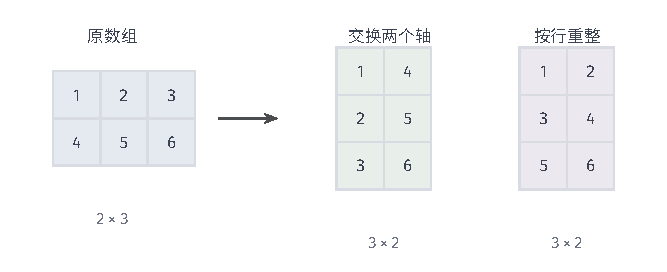
\includegraphics[width=112mm]{figures/01-mathematical-preliminaries-upper/02-linear-spaces/tikz/comprehension-additions/linear-transpose-reshape.pdf}
  \caption{轴交换与按行重整。原数组两行为$(1,2,3)$与$(4,5,6)$；中图转置后两列分别保留原来的两行，右图则把按行读取的数列$1,2,3,4,5,6$依次装入$3\times2$数组。数字及其排列由正文示例直接给出。}
  \label{fig:vol1-add-linear-transpose-reshape}
\end{figure}

\paragraph{向量化}

按列堆叠的\term{向量化}（vectorization）把$m\times n$矩阵展成长列：
\[
 \operatorname{vec}(\bm A)=(a_{1,1},\ldots,a_{m,1},a_{1,2},\ldots,a_{m,n})^\top,
\]
元素$a_{i,j}$对应一维索引$i+(j-1)m$。反过来，矩阵展开（unfolding）把多维数组的指定轴选为行、其余轴合并为列，得到一个矩阵；选哪些轴保留为独立索引，决定展开结果的形状，也决定后续乘积汇总哪个轴。向量化与展开都是固定索引映射的reshape，保留全部信息。

\subsection{运算性质}

目标形状与遍历顺序固定后，转置、轴置换、reshape与向量化都是数组空间之间的线性双射：它们把加法和数乘逐项搬到新排列，逆变换（再转置一次、逆置换、按原次序装回）恢复原数组。因此$(\bm A+\bm B)^\top=\bm A^\top+\bm B^\top$、$(c\bm A)^\top=c\bm A^\top$一类等式按位置直接成立。

转置与乘法的交互由元素公式推出：
\[
 (\bm A^\top)^\top=\bm A,\qquad
 (\bm A\bm B)^\top=\bm B^\top\bm A^\top,\qquad
 (\bm A^{-1})^\top=(\bm A^\top)^{-1}.
\]
乘积转置后因子次序反转；可逆矩阵转置后仍可逆，逆与转置可交换次序。转置还保持矩阵秩，因为行空间与列空间只是互换。一般reshape不保持矩阵秩：它只重排元素，新矩阵各行各列之间的线性相关关系可以完全不同。轴置换与reshape都不是映射作用，把存储格式当成几何性质或变换效果，是这里最常见的错误。

\section{内积}
\label{sec:ls-inner-products}

加法与乘法回答怎样合并对象，内积则把两个对象配成一个标量：它同时给出长度、角度和垂直的判据。第~\ref{chap:sets-functions-and-proofs}章已在标准坐标下定义$\langle\bm x,\bm y\rangle=\sum_j x_jy_j$，本节先把它抽象为配对公理，再引入区分方向代价的加权配对，最后用Gram矩阵建立正交分解和线性泛函的内积表示。

\subsection{内积的定义与性质}

\paragraph{内积的定义}

\begin{definition}[实内积]
\label{def:linear-algebra-inner-product}
\label{def:functional-inner-product-space}
实向量空间$V$上的\term{内积}（inner product）是映射$\langle\cdot,\cdot\rangle:V\times V\to\mathbb R$，同时满足下列三条公理。
\begin{enumerate}
 \item 双线性：对两个变量分别保持线性组合，即$\langle a\bm x+b\bm y,\bm z\rangle=a\langle\bm x,\bm z\rangle+b\langle\bm y,\bm z\rangle$，且对第二变量同样线性。
 \item 对称性：$\langle\bm x,\bm y\rangle=\langle\bm y,\bm x\rangle$。
 \item 正定性：$\langle\bm x,\bm x\rangle>0$对所有非零$\bm x$成立，且$\langle\bm x,\bm x\rangle=0$当且仅当$\bm x=\bm0$。
\end{enumerate}
配备内积的向量空间称为\term{内积空间}（inner-product space）。
\end{definition}

标准实坐标的内积是$\langle\bm x,\bm y\rangle=\bm x^\top\bm y=\sum_j x_jy_j$。由配对直接诱导长度
\begin{equation}
 \lVert\bm x\rVert=\sqrt{\langle\bm x,\bm x\rangle},
 \label{eq:linear-algebra-inner-product-norm}
\end{equation}
$\langle\bm x,\bm y\rangle=0$时称两向量\term{正交}（orthogonal）。

\paragraph{Cauchy--Schwarz不等式}

内积能否给出夹角，取决于配对值是否受两个长度控制。
\begin{theorem}[Cauchy--Schwarz不等式]
\label{thm:linear-algebra-cauchy-schwarz}
在内积空间中，$|\langle\bm x,\bm y\rangle|\leq\lVert\bm x\rVert\,\lVert\bm y\rVert$，等号成立当且仅当两向量线性相关。
\end{theorem}
\begin{proof}
$\bm y=\bm0$时两边都为零。否则令$a=\langle\bm x,\bm y\rangle/\lVert\bm y\rVert^2$，则
\[
 0\leq\lVert\bm x-a\bm y\rVert^2
 =\lVert\bm x\rVert^2-\frac{\langle\bm x,\bm y\rangle^2}{\lVert\bm y\rVert^2}.
\]
移项即得不等式；等号恰好要求$\bm x-a\bm y=\bm0$，即两向量共线。
\end{proof}

非零向量的夹角由$\cos\theta=\langle\bm x,\bm y\rangle/(\lVert\bm x\rVert\lVert\bm y\rVert)$定义，CS不等式保证它落在$[-1,1]$。例如$\bm x=(1,0)^\top$、$\bm y_\varepsilon=(1,\varepsilon)^\top$随$\varepsilon\to0$趋近共线，
\begin{equation}
 \cos\theta_\varepsilon=\frac{1}{\sqrt{1+\varepsilon^2}}\longrightarrow1,
 \label{eq:linear-algebra-nearly-collinear-angle}
\end{equation}
这给“几乎同向”一个确定的欧氏度量；更换内积也会更换角度。

并非每个范数都来自内积。实向量空间中一个范数来自内积，当且仅当它满足\term{平行四边形恒等式}
\begin{equation}
 \lVert\bm x+\bm y\rVert^2+\lVert\bm x-\bm y\rVert^2
 =2\lVert\bm x\rVert^2+2\lVert\bm y\rVert^2.
 \label{eq:functional-parallelogram-identity}
\end{equation}
必要性由内积展开直接得到；例如第~\ref{sec:ls-norms-distances}节的$\ell_1$范数在$\bm e_1,\bm e_2$上左侧为$8$、右侧为$4$，故不来自任何内积。充分性可用极化公式$\langle\bm x,\bm y\rangle=(\lVert\bm x+\bm y\rVert^2-\lVert\bm x-\bm y\rVert^2)/4$恢复配对，这里不展开。

对同形矩阵，把元素看作有限坐标，得到\term{Frobenius内积}
\[
 \langle\bm A,\bm B\rangle_{\mathrm F}=\sum_{i,j}a_{i,j}b_{i,j},
 \qquad
 \lVert\bm A\rVert_{\mathrm F}=\left(\sum_{i,j}a_{i,j}^2\right)^{1/2}.
\]
这是矩阵作为数表本身的长度；它与矩阵作为变换时的最大放大率不是同一口径，后者在第~\ref{sec:ls-matrix-norms}节建立。

\subsection{加权内积}
\label{sec:ls-weighted-inner-products}

标准坐标把每个方向一视同仁，但实际问题里不同方向的代价不同。设$\bm M=\operatorname{diag}(4,1)$，则$\sqrt{4x_1^2+x_2^2}$把第一坐标的偏差放大两倍：点$(1,1)$的欧氏长度是$\sqrt2$，这种加权长度却是$\sqrt5$。只要权重矩阵满足适当条件，这样的长度仍来自一个合法内积。

对称矩阵$\bm M$给出二次型$q(\bm x)=\bm x^\top\bm M\bm x$：若对每个非零$\bm x$都有$q(\bm x)>0$，称$\bm M$\term{正定}（positive definite）；若只保证$q(\bm x)\geq0$，称$\bm M$\term{半正定}（positive semidefinite）。要求对称，是因为配对必须对称；非对称部分在$\bm x^\top\bm M\bm x$中自动抵消，不进入二次型。

\paragraph{加权内积的定义}

对称正定$\bm M$给出加权配对
\[
 \langle\bm x,\bm y\rangle_{\bm M}=\bm x^\top\bm M\bm y,
 \qquad
 \lVert\bm x\rVert_{\bm M}=\sqrt{\bm x^\top\bm M\bm x}.
\]
它满足双线性、对称与正定性，是一个合法内积。若$\bm M$仅半正定，配对只给半内积，诱导半范数以及伪距离
\begin{equation}
 d_{\bm M}(\bm x,\bm y)
 =\sqrt{(\bm x-\bm y)^\top\bm M(\bm x-\bm y)}.
 \label{eq:linear-algebra-mahalanobis-pseudodistance}
\end{equation}
不同点的距离可能为零：例如$\bm M=\operatorname{diag}(1,0)$无法区分$(0,0)^\top$与$(0,1)^\top$。半正定时CS不等式仍可由$\langle\bm x+t\bm y,\bm x+t\bm y\rangle_{\bm M}\geq0$对所有实数$t$成立得到，三角不等式保留。

\paragraph{Gram因子定理}

加权配对不必当作新几何：有限维半正定矩阵都能写成欧氏平方和。
\begin{theorem}[半正定矩阵的配方因子]
\label{thm:ls-gram-factor}
设$\bm M\in\mathbb R^{r\times r}$对称半正定，则存在$\bm L$使$\bm M=\bm L^\top\bm L$；若$\bm M$正定，可取$\bm L$可逆。
\end{theorem}
\begin{proof}
对$r$归纳。$r=1$时$\bm M=(m_{1,1})$且$m_{1,1}\geq0$，取$\bm L=(\sqrt{m_{1,1}})$即可。

若所有对角项都为零，任取$i,j$，把$\bm x=\bm e_i+t\bm e_j$代入半正定性：
\[
 0\leq\bm x^\top\bm M\bm x=2t\,m_{i,j}+t^2m_{j,j}=2t\,m_{i,j},
\]
对正负$t$同时成立迫使$m_{i,j}=0$，于是$\bm M=0$，取$\bm L=0$。

否则存在正对角项。取一个置换矩阵$\bm P$（行列同步交换，$\bm P^\top=\bm P^{-1}$）把它换到首位，记
\[
 \widetilde{\bm M}=\bm P\bm M\bm P^\top
 =\begin{bmatrix}a&\bm b^\top\\ \bm b&\bm C\end{bmatrix},\qquad a>0.
\]
配方消去第一行：令$\bm x=(-\bm b^\top\bm u/a,\bm u)$，则$\bm x^\top\widetilde{\bm M}\bm x=\bm u^\top(\bm C-\bm b\bm b^\top/a)\bm u\geq0$，故余项$\bm M'=\bm C-\bm b\bm b^\top/a$仍半正定。由归纳假设$\bm M'=\bm L'^\top\bm L'$，取上三角因子
\[
 \widetilde{\bm L}=\begin{bmatrix}\sqrt a&\bm b^\top/\sqrt a\\ \bm0&\bm L'\end{bmatrix},
\]
直接相乘得
\[
 \widetilde{\bm L}^\top\widetilde{\bm L}
 =\begin{bmatrix}a&\bm b^\top\\ \bm b&\bm b\bm b^\top/a+\bm L'^\top\bm L'\end{bmatrix}
 =\widetilde{\bm M}.
\]
换回原矩阵：$\bm M=\bm P^\top\widetilde{\bm M}\bm P=(\widetilde{\bm L}\bm P)^\top(\widetilde{\bm L}\bm P)$，取$\bm L=\widetilde{\bm L}\bm P$即可。

正定时$\bm M'$也正定（上述$\bm x$在$\bm u\neq\bm0$时非零），归纳得$\bm L'$可逆，于是$\widetilde{\bm L}$可逆，$\bm L=\widetilde{\bm L}\bm P$仍可逆。
\end{proof}
于是加权长度可写成$\lVert\bm x\rVert_{\bm M}=\lVert\bm L\bm x\rVert_2$：正定时只是换了一组坐标，退化时则把$\bm L$的零空间方向压成零长度。使用半内积前必须先说明哪些方向被忽略，不能把退化配对当成正定内积参与正交判断。证明中的配方步骤就是第~\ref{sec:ls-exact-linear-equations}节Cholesky分解的雏形。

对两个对称矩阵记$\bm M\succeq\bm N$当且仅当$\bm M-\bm N$半正定，即$\bm x^\top\bm M\bm x\geq\bm x^\top\bm N\bm x$对所有$\bm x$成立，它给出加权长度的逐点比较$\lVert\bm x\rVert_{\bm M}\geq\lVert\bm x\rVert_{\bm N}$。作可逆线性替换$\bm x=\bm S\bm z$，二次型变为$\bm z^\top(\bm S^\top\bm M\bm S)\bm z$；这种合同变换$\bm M\mapsto\bm S^\top\bm M\bm S$保持半正定性、正定性与序关系。因此换基后新坐标下的度量矩阵是$\bm S^\top\bm M\bm S$而不是$\bm M$，把新坐标直接按欧氏长度比较，一般已经换了问题。

\subsection{正交关系}
\label{sec:ls-orthogonality}

\paragraph{Gram矩阵}

正交是两个向量之间的关系；一组向量之间的全部配对关系由一张数表记录。
\begin{definition}[有限向量族的Gram矩阵]
\label{def:linear-algebra-gram-matrix}
向量$\bm b_1,\ldots,\bm b_r$的\term{Gram矩阵}（Gram matrix）为$g_{i,j}=\langle\bm b_i,\bm b_j\rangle$。若$\bm B$以它们为列，标准坐标中$\bm G=\bm B^\top\bm B$，加权坐标中$\bm G=\bm B^\top\bm M\bm B$。
\end{definition}

因为$\bm a^\top\bm G\bm a=\lVert\sum_j a_j\bm b_j\rVert^2\geq0$，Gram矩阵半正定；并且$\bm G$正定（从而非奇异）当且仅当这组向量线性无关：线性相关时某个非零系数使组合为零，平方长度为零；线性无关时任意非零系数的组合非零，平方长度为正。$\bm G$是对角阵恰好表示这组向量两两正交，是单位阵则表示两两正交且长度为$1$。图~\ref{fig:ls-gram-matrix-coefficients} 把两条基向量的两两内积排成数表。
\begin{figure}[!htb]
  \centering
  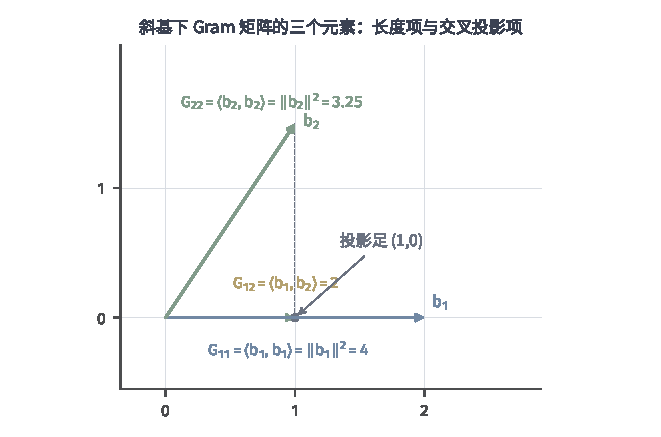
\includegraphics[width=112mm]{figures/01-mathematical-preliminaries-upper/02-linear-spaces/matplotlib/ls-gram-matrix-coefficients/ls-gram-matrix-coefficients.pdf}
  \caption{Gram矩阵把一组基向量的两两内积排成数表。左：平面上两条不垂直的基向量$\bm b_1,\bm b_2$及其夹角；右：$G_{i,j}=\langle\bm b_i,\bm b_j\rangle$构成的$2\times2$Gram矩阵，对角元为各向量长度平方，非对角元为夹角投影。基越接近正交，非对角元越接近零；线性相关时$\det\bm G=0$。向量与矩阵均为解析教学例。}
  \label{fig:ls-gram-matrix-coefficients}
\end{figure}

\paragraph{正交补与正交直和}

设$U$是有限维内积空间$V$的子空间，\term{正交补}（orthogonal complement）定义为
\[
 U^\perp=\{\bm r\in V:\langle\bm u,\bm r\rangle=0,\ \forall\bm u\in U\}.
\]
Gram矩阵非奇异给出正交分解的存在与唯一。
\begin{lemma}[正交直和]
\label{lem:ls-orthogonal-decomposition}
设$U$是有限维内积空间$V$的子空间，则每个$\bm x\in V$唯一分解为$\bm x=\bm u+\bm r$，其中$\bm u\in U$、$\bm r\in U^\perp$；即$V=U\oplus U^\perp$。
\end{lemma}
\begin{proof}
取$U$的一组基$\bm b_1,\ldots,\bm b_r$，其Gram矩阵$\bm G$非奇异。对任意$\bm x$，令$\bm u=\sum_j a_j\bm b_j$，并要求$\bm r=\bm x-\bm u$与每个$\bm b_i$正交，得到系数方程
\[
 \sum_j g_{i,j}a_j=\langle\bm b_i,\bm x\rangle,\qquad i=1,\ldots,r,
\]
即$\bm G\bm a=(\langle\bm b_i,\bm x\rangle)_i$。非奇异$\bm G$保证系数唯一解出，残差$\bm r$与全部基向量正交，因而落在$U^\perp$。

若$\bm x=\bm u+\bm r=\bm u'+\bm r'$是两种分解，则$\bm u-\bm u'=\bm r'-\bm r$同时属于$U$与$U^\perp$，与自身正交，长度为零，故两种分解相同。
\end{proof}
这里只证明正交分量存在且唯一；它就是$U$中离$\bm x$最近的点，这一判定与具体算法在第~\ref{sec:ls-subspace-nearest-points}节给出。

\section{范数与距离}
\label{sec:ls-norms-distances}
\label{sec:linear-algebra-distance-relations}
\label{sec:ch06-map-comparison}
\label{sec:matrix-analysis-norms-effective-rank}
\label{sec:linear-algebra-length-angle-distance}

同一个误差向量$(1,1)$可以按绝对偏差计为$2$，按欧氏长度计为$\sqrt2$，也可以只记录最大坐标偏差$1$。不同任务要求不同的误差含义，没有对所有目的都最合适的长度。本节用范数统一表达这些尺度，再给出矩阵的大小、点间的距离与夹角，以及线性读取在给定误差预算下的最大值。

\subsection{向量范数}

\paragraph{范数的定义}

\begin{definition}[赋范空间]
\label{def:functional-normed-space}
设$V$为实向量空间。映射$\lVert\cdot\rVert:V\to[0,\infty)$同时满足下列四条公理时，称为\term{范数}（norm），$(V,\lVert\cdot\rVert)$称为\term{赋范空间}（normed space）。它诱导距离$d(\bm x,\bm y)=\lVert\bm x-\bm y\rVert$。
\begin{enumerate}
 \item 非负性：$\lVert\bm x\rVert\geq0$。
 \item 正定性：$\lVert\bm x\rVert=0$当且仅当$\bm x=\bm0$。
 \item 齐次性：$\lVert c\bm x\rVert=|c|\,\lVert\bm x\rVert$。
 \item 三角不等式：$\lVert\bm x+\bm y\rVert\leq\lVert\bm x\rVert+\lVert\bm y\rVert$。
\end{enumerate}
\end{definition}

内积诱导的$\lVert\bm x\rVert=\sqrt{\langle\bm x,\bm x\rangle}$满足公理：正定性直接来自内积，三角不等式由$\lVert\bm x+\bm y\rVert^2=\lVert\bm x\rVert^2+2\langle\bm x,\bm y\rangle+\lVert\bm y\rVert^2$和CS不等式得到。

有限坐标中常用
\[
 \lVert\bm x\rVert_p=\left(\sum_j|x_j|^p\right)^{1/p}\quad(1\leq p<\infty),
 \qquad
 \lVert\bm x\rVert_\infty=\max_j|x_j|.
\]
$p=1$累加绝对偏差，$p=2$累计平方偏差再开方，$p=\infty$控制最大坐标偏差。图~\ref{fig:ls-norm-unit-balls} 比较三种口径下单位球的形状。
\begin{figure*}[htbp]
  \centering
  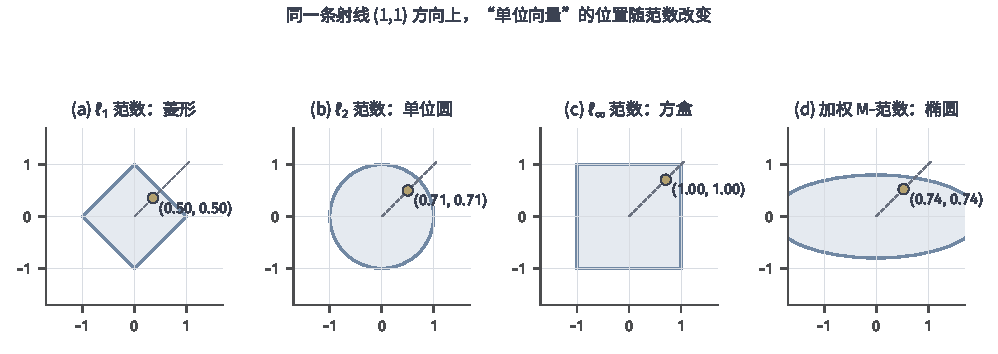
\includegraphics[width=169mm]{figures/01-mathematical-preliminaries-upper/02-linear-spaces/matplotlib/ls-norm-unit-balls/ls-norm-unit-balls.pdf}
  \caption{同一向量在不同范数下的“单位球”形状。左：$\ell_1$单位球为菱形（累加绝对偏差）；中：$\ell_2$单位球为圆（欧氏长度）；右：$\ell_\infty$单位球为正方形（最大坐标偏差）。同一个点$(1,1)$的范数依次为$2$、$\sqrt2$、$1$，单位球大小随口径而变，三者之间的倍数关系由正文的显式不等式给出。三图坐标尺度相同，为解析教学例。}
  \label{fig:ls-norm-unit-balls}
\end{figure*}

$p=1,2,\infty$的三角不等式可以直接验证；一般$p$需要下面的不等式。
\begin{theorem}[有限维Hölder不等式]
\label{thm:linear-algebra-holder}
设$1\leq p,q\leq\infty$且$1/p+1/q=1$（约定$1/\infty=0$），则$|\bm x^\top\bm y|\leq\lVert\bm x\rVert_p\lVert\bm y\rVert_q$。
\end{theorem}
\begin{proof}
先设$1<p,q<\infty$。Young不等式$uv\leq u^p/p+v^q/q$对$u,v\geq0$成立：$u>0$时令$t=v/u^{p-1}$，验证$1/p+t^q/q-t\geq0$，其最小值在$t=1$处为零；$u=0$时也成立。两向量非零时取$u_j=|x_j|/\lVert\bm x\rVert_p$、$v_j=|y_j|/\lVert\bm y\rVert_q$求和，得$\sum_j u_jv_j\leq1/p+1/q=1$，恢复尺度后用$|\bm x^\top\bm y|\leq\sum_j|x_j||y_j|$。零向量时两侧都为零；$p=1,q=\infty$时用$\sum_j|x_j||y_j|\leq(\max_j|y_j|)\sum_j|x_j|$，另一端点交换两者。
\end{proof}
对一般$p$，把$|x_j+y_j|^{p}\leq|x_j+y_j|^{p-1}(|x_j|+|y_j|)$求和后对两部分分别应用Hölder，得到
$\lVert\bm x+\bm y\rVert_p^p\leq(\lVert\bm x\rVert_p+\lVert\bm y\rVert_p)\lVert\bm x+\bm y\rVert_p^{p-1}$，非零时相除即得三角不等式（Minkowski不等式）。常用坐标范数之间还有直接界
\[
 \lVert\bm x\rVert_\infty\leq\lVert\bm x\rVert_2\leq\sqrt d\,\lVert\bm x\rVert_\infty,
 \qquad
 \lVert\bm x\rVert_2\leq\lVert\bm x\rVert_1\leq\sqrt d\,\lVert\bm x\rVert_2,
\]
右端两式分别来自$\sum_jx_j^2\leq d\max_jx_j^2$与Cauchy--Schwarz不等式。维数增大时$\sqrt d$不能在误差预算中忽略。

分组误差要先固定分组方式，例如以行为组的混合范数
$\lVert\bm A\rVert_{p,q}=(\sum_i\lVert\bm A_{i,:}\rVert_p^q)^{1/q}$，内层衡量组内、外层汇总各组。允许非零对象也具有零大小、但保留齐次性与三角不等式的尺度称为\term{半范数}（seminorm），它给出伪距离：例如只读取截距的仿射函数尺度$p(f_{a,b})=|a|$忽略全部斜率方向，相同截距的不同函数距离为零。把零方向归并为同一元素后得到的商范数，在讨论点到子空间的距离时给出（第~\ref{sec:ls-quotient-norms}节）。

\subsection{矩阵范数}
\label{sec:ls-matrix-norms}

矩阵有两种“大小”口径：Frobenius范数描述数表本身有多大；误差分析更关心它作为变换最坏把输入放大多少倍。
\begin{definition}[由向量范数诱导的矩阵范数]
\label{def:matrix-analysis-induced-norm}
给定输入范数$\lVert\cdot\rVert_\alpha$和输出范数$\lVert\cdot\rVert_\beta$，\term{诱导矩阵范数}（induced matrix norm）为
\[
 \lVert\bm A\rVert_{\alpha\to\beta}
 =\sup_{\bm x\neq0}\frac{\lVert\bm A\bm x\rVert_\beta}{\lVert\bm x\rVert_\alpha}.
\]
两端采用同一类$p$范数时简写为$\lVert\bm A\rVert_p$。
\end{definition}

\paragraph{诱导矩阵范数}

由定义直接得$\lVert\bm A\bm x\rVert_\beta\leq\lVert\bm A\rVert_{\alpha\to\beta}\lVert\bm x\rVert_\alpha$，诱导范数就是这一不等式中最小的常数。标准坐标下两个诱导范数可直接读取：
\[
 \lVert\bm A\rVert_1=\max_j\sum_i|a_{i,j}|,\qquad
 \lVert\bm A\rVert_\infty=\max_i\sum_j|a_{i,j}|.
\]
第一式由$\lVert\bm A\bm x\rVert_1\leq\sum_j|x_j|\lVert\bm A_{:,j}\rVert_1$得到上界，在最大绝对列和对应的坐标向量上达到；第二式的上界同理，取输入各坐标为对应行元素的符号即达到。诱导$2$范数也称\term{谱范数}（spectral norm），$\lVert\bm A\rVert_2=\sup_{\lVert\bm x\rVert_2=1}\lVert\bm A\bm x\rVert_2$；对每行用CS不等式得$\lVert\bm A\bm x\rVert_2\leq\lVert\bm A\rVert_{\mathrm F}\lVert\bm x\rVert_2$，故它有限且$\lVert\bm A\rVert_2\leq\lVert\bm A\rVert_{\mathrm F}$，其奇异值表达在第~\ref{sec:ls-svd}节推导。对一般的范数对，比值有界且上确界在某个方向达到，由第~\ref{sec:ls-error-scale-comparison}节的范数等价与极值定理保证。图~\ref{fig:ls-induced-norm-action} 把单位圆被拉成椭圆后的最长轴读作最大放大倍数。
\begin{figure*}[htbp]
  \centering
  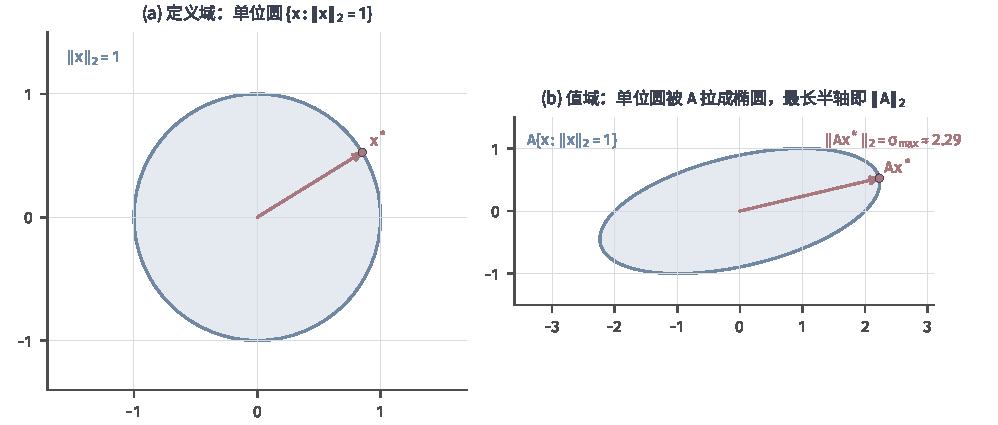
\includegraphics[width=169mm]{figures/01-mathematical-preliminaries-upper/02-linear-spaces/matplotlib/ls-induced-norm-action/ls-induced-norm-action.pdf}
  \caption{诱导矩阵范数衡量最坏放大倍数。左：单位圆$\lVert\bm x\rVert_2=1$；中：同一线性作用$\bm A$把单位圆映成椭圆；右：椭圆上最长的轴给出$\lVert\bm A\rVert_2=\max_{\lVert\bm x\rVert_2=1}\lVert\bm A\bm x\rVert_2$，箭头指示最大放大方向。数值由$\bm A$的教学构造直接得到，是解析例。}
  \label{fig:ls-induced-norm-action}
\end{figure*}

Frobenius范数从另一个角度累计作用：
\[
 \lVert\bm A\rVert_{\mathrm F}^2
 =\sum_j\lVert\bm A\bm e_j\rVert_2^2
 =\sum_{i,j}a_{i,j}^2,
\]
它是所有标准输入方向的总平方输出，而非一次最坏输入。对$\bm A=\begin{smallmatrix}1&1\\0&1\end{smallmatrix}$，$\lVert\bm A\rVert_1=\lVert\bm A\rVert_\infty=2$、$\lVert\bm A\rVert_{\mathrm F}=\sqrt3$，不同口径的数值不必相同。

中间空间范数匹配时，连续应用两次界得到次乘性
\[
 \lVert\bm A\bm B\rVert_{\alpha\to\gamma}
 \leq\lVert\bm A\rVert_{\beta\to\gamma}
 \lVert\bm B\rVert_{\alpha\to\beta}.
\]
逐列应用诱导范数界，转置后对列重复同一论证，得到混合界
\begin{equation}
 \lVert\bm A\bm B\rVert_{\mathrm F}
 \leq\lVert\bm A\rVert_2\lVert\bm B\rVert_{\mathrm F},
 \qquad
 \lVert\bm A\bm B\rVert_{\mathrm F}
 \leq\lVert\bm A\rVert_{\mathrm F}\lVert\bm B\rVert_2.
 \label{eq:matrix-analysis-mixed-submultiplicativity}
\end{equation}
其中$\lVert\bm B^\top\rVert_2=\lVert\bm B\rVert_2$可由
$\lVert\bm B\rVert_2=\max_{\lVert\bm x\rVert_2=\lVert\bm y\rVert_2=1}|\bm y^\top\bm B\bm x|$交换两向量得到。结合$\lVert\bm A\rVert_2\leq\lVert\bm A\rVert_{\mathrm F}$，Frobenius范数也次乘。

\subsection{距离与夹角}

范数诱导的距离$d(\bm x,\bm y)=\lVert\bm x-\bm y\rVert$满足非负、对称与三角不等式；非零向量的夹角已由CS不等式在第~\ref{sec:ls-inner-products}节定义。更换范数只改变距离口径，不改变两点是否重合。

比较两个方向时先把各自归一化到单位长度，消除整体缩放：$\bm x$与$c\bm x$（$c\neq0$）是同一方向，$\langle\bm x/\lVert\bm x\rVert,\bm y/\lVert\bm y\rVert\rangle$才只反映角度。两个子空间之间的夹角以各自单位向量之间的最小夹角为起点定义，其计算与敏感度在后续分析章节展开。尺度约定不同（例如一边用$\ell_2$、一边用$\ell_1$又不归一）时，比较结果没有意义，因此先统一度量口径再谈远近。

\subsection{对偶范数}
\label{sec:ls-dual-norms}

\paragraph{对偶范数}

误差$\bm r$只知道落在某个范数球内时，一次线性读取$\bm z^\top\bm r$最多变化多少，由下面的量回答。
\begin{definition}[对偶范数]
\label{def:linear-algebra-dual-norm}
给定$\mathbb R^d$上的范数，相对于标准坐标配对的\term{对偶范数}（dual norm）为
\begin{equation}
 \lVert\bm z\rVert_*=\sup_{\lVert\bm r\rVert\leq1}|\bm z^\top\bm r|.
 \label{eq:linear-algebra-dual-norm-definition}
\end{equation}
\end{definition}
它满足范数公理：线性读取满足三角不等式与齐次性，非零$\bm z$总能读取某个坐标得到非零值。对$\ell_p$范数，下面直接构造达到上确界的$\bm r$；一般范数下上确界同样可以取到（第~\ref{sec:ls-error-scale-comparison}节）。图~\ref{fig:ls-dual-norm-unit-ball} 把这个最大值画成支撑线最后接触单位球的位置。

\begin{figure}[!htb]
  \centering
  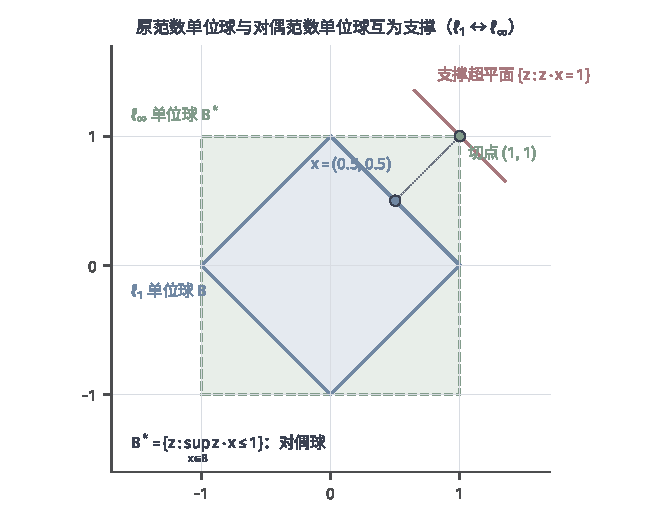
\includegraphics[width=112mm]{figures/01-mathematical-preliminaries-upper/02-linear-spaces/matplotlib/ls-dual-norm-unit-ball/ls-dual-norm-unit-ball.pdf}
  \caption{对偶范数的几何：在原范数单位球$\lVert\bm r\rVert\leq1$上求线性读取$\bm z^\top\bm r$的最大值。左：原单位球（灰色）与读取方向$\bm z$；右：支撑直线最后接触单位球处给出$\lVert\bm z\rVert_*=\max_{\lVert\bm r\rVert\leq1}|\bm z^\top\bm r|$。对偶单位球（虚线）与原单位球互为极体，为解析教学例。}
  \label{fig:ls-dual-norm-unit-ball}
\end{figure}

Hölder不等式给出$\ell_p$单位球上的上界$\lVert\bm z\rVert_q$，且上界可达到：$1<p<\infty$时取$r_j=|z_j|^{q-1}\operatorname{sgn}(z_j)/\lVert\bm z\rVert_q^{q-1}$；$p=1$时把单位预算放在$|z_j|$最大的坐标；$p=\infty$时逐坐标取$r_j=\operatorname{sgn}(z_j)$。因而
\begin{equation}
 (\lVert\cdot\rVert_p)_*=\lVert\cdot\rVert_q,\qquad \frac1p+\frac1q=1,
 \label{eq:linear-algebra-lp-duality}
\end{equation}
并对$\rho\geq0$有
\begin{equation}
 \max_{\lVert\bm r\rVert_p\leq\rho}|\bm z^\top\bm r|
 =\rho\lVert\bm z\rVert_q.
 \label{eq:linear-algebra-linear-perturbation-duality}
\end{equation}
例如$\bm z=(2,-1)^\top$、$|r_j|\leq0.01$时最大变化为$0.03$，由$\bm r=(0.01,-0.01)^\top$达到。图~\ref{fig:linear-algebra-dual-unit-balls} 固定同一次读取，显示预算形状怎样改变最坏方向。
\begin{figure*}[htbp]
  \centering
  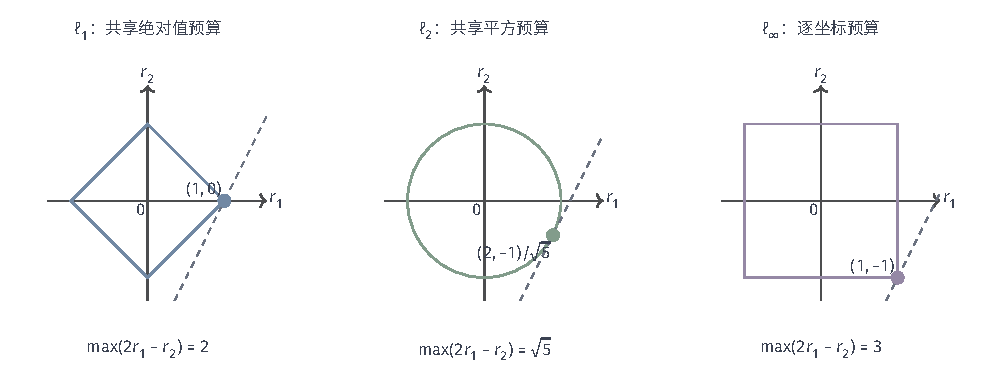
\includegraphics[width=168.998mm]{figures/01-mathematical-preliminaries-upper/02-linear-spaces/tikz/linear-algebra-dual-unit-balls/figure.pdf}
  \caption{同一线性读取$2r_1-r_2$在$\ell_1$、$\ell_2$、$\ell_\infty$单位球上的最大值依次为$2$、$\sqrt5$、$3$。虚线为最后接触可行集的支撑直线，点为最大化方向。三图坐标尺度相同，均为解析教学例；改变允许误差的形状会改变误差常数。}
  \label{fig:linear-algebra-dual-unit-balls}
\end{figure*}

加权长度$\lVert\bm r\rVert_{\bm M}=\sqrt{\bm r^\top\bm M\bm r}$的对偶范数由逆矩阵给出：误差按$\bm M$计量时，读取方向要按$\bm M^{-1}$计量。
\begin{theorem}[加权对偶范数]
\label{prop:ls-weighted-dual-norm}
设$\bm M$对称正定，则范数$\lVert\cdot\rVert_{\bm M}$相对于标准坐标配对的对偶范数为
\[
 \lVert\bm z\rVert_{\bm M,*}
 =\sup_{\bm r^\top\bm M\bm r\leq1}\bm z^\top\bm r
 =\sqrt{\bm z^\top\bm M^{-1}\bm z}.
\]
\end{theorem}
\begin{proof}
取可逆配方因子$\bm M=\bm L^\top\bm L$（定理~\ref{thm:ls-gram-factor}），令$\bm w=\bm L\bm r$，约束化为$\bm w^\top\bm w\leq1$，目标化为$\bm z^\top\bm r=\bm z^\top\bm L^{-1}\bm w=(\bm L^{-\top}\bm z)^\top\bm w$。由欧氏情形$\sup_{\lVert\bm w\rVert_2\leq1}\bm a^\top\bm w=\lVert\bm a\rVert_2$（$\bm w=\bm a/\lVert\bm a\rVert_2$时取到），上确界为
\[
 \lVert\bm L^{-\top}\bm z\rVert_2
 =\sqrt{\bm z^\top\bm L^{-1}\bm L^{-\top}\bm z}
 =\sqrt{\bm z^\top\bm M^{-1}\bm z},
\]
其中$\bm L^{-1}\bm L^{-\top}=(\bm L^\top\bm L)^{-1}=\bm M^{-1}$。
\end{proof}

把约束中的$\bm r$按比例缩放，定理也可写成$\bm z^\top\bm M^{-1}\bm z=\sup_{\bm r\neq\bm0}(\bm z^\top\bm r)^2/(\bm r^\top\bm M\bm r)$。由这一极值写法立即得到正定矩阵求逆的序反转。
\begin{theorem}[正定求逆的序反转]
\label{cor:ls-inverse-order-reversal}
若$\bm M_1\preceq\bm M_2$都正定，则$\bm M_2^{-1}\preceq\bm M_1^{-1}$。
\end{theorem}
\begin{proof}
对任意$\bm z$，由$\bm r^\top\bm M_1\bm r\leq\bm r^\top\bm M_2\bm r$，分母较小者比值较大：
\[
 \bm z^\top\bm M_2^{-1}\bm z
 =\sup_{\bm r\neq\bm0}\frac{(\bm z^\top\bm r)^2}{\bm r^\top\bm M_2\bm r}
 \leq\sup_{\bm r\neq\bm0}\frac{(\bm z^\top\bm r)^2}{\bm r^\top\bm M_1\bm r}
 =\bm z^\top\bm M_1^{-1}\bm z.
\]
\end{proof}
原度量增大时，对偶度量缩小。这是两个对称矩阵之间的序关系，不是逐元素不等式。

\section{伴随}
\label{sec:ls-adjoints}

矩阵转置把作用从输出端搬回输入端，但“搬运”依赖所选配对。内积空间中这个搬运者称为伴随；它与代数对偶中的转置、与求解复原的逆是三个不同对象。

\subsection{定义与性质}

\paragraph{内积伴随的定义}

设$T:V\to W$是两个有限维实内积空间之间的线性映射。若存在$T^\star:W\to V$使
\begin{equation}
 \langle T\bm x,\bm y\rangle_W=\langle\bm x,T^\star\bm y\rangle_V
 \label{eq:ls-adjoint-pairing}
\end{equation}
对所有$\bm x\in V$、$\bm y\in W$成立，则$T^\star$称为$T$的\term{伴随}（adjoint）。
\label{def:linear-algebra-adjoint}

伴随总存在且唯一。取$V,W$的基，把两边的内积写成$\langle\bm x,\bm x'\rangle_V=\bm x^\top\bm M_V\bm x'$、$\langle\bm y,\bm y'\rangle_W=\bm y^\top\bm M_W\bm y'$，其中$\bm M_V,\bm M_W$是基的Gram矩阵，对称正定因而可逆；设$T$的矩阵为$\bm A$，所求伴随的矩阵为$\bm B$。式~\eqref{eq:ls-adjoint-pairing}要求$(\bm A\bm x)^\top\bm M_W\bm y=\bm x^\top\bm M_V\bm B\bm y$对所有$\bm x,\bm y$成立，即$\bm A^\top\bm M_W=\bm M_V\bm B$，它有唯一解
\begin{equation}
 \bm B=\bm M_V^{-1}\bm A^\top\bm M_W.
 \label{eq:ls-weighted-adjoint}
\end{equation}
标准内积下$\bm M_V,\bm M_W$都是单位矩阵，伴随矩阵就是$\bm A^\top$；两边权重不同时，伴随既不是单纯转置，也不是转置再求逆。

伴随与组合的规则由配对定义逐项推出：
\[
 (T+S)^\star=T^\star+S^\star,\qquad
 (cT)^\star=c\,T^\star,\qquad
 (TS)^\star=S^\star T^\star,\qquad
 T^{\star\star}=T.
\]
复合伴随的次序与乘积转置一样反转；恒等映射的伴随是自身。图~\ref{fig:ls-adjoint-action-transfer} 把这种配对方向的搬回画成示意图。
\begin{figure}[!htb]
  \centering
  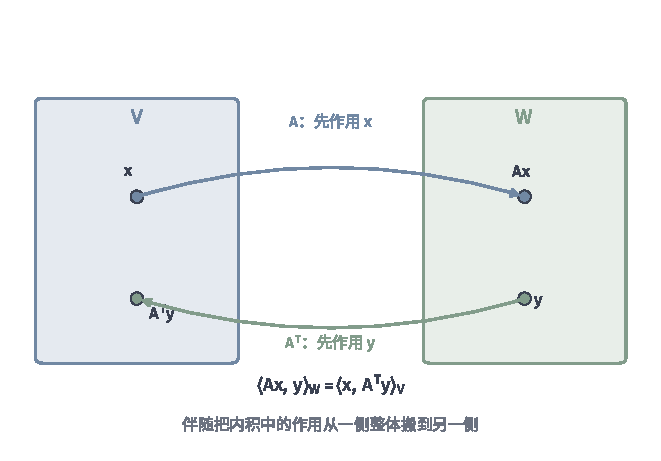
\includegraphics[width=112mm]{figures/01-mathematical-preliminaries-upper/02-linear-spaces/matplotlib/ls-adjoint-action-transfer/ls-adjoint-action-transfer.pdf}
  \caption{内积伴随把输出端的配对搬回输入端。左：$T:V\to W$把$\bm x$映成$T\bm x$，与$\bm y\in W$配对；右：伴随$T^\star:W\to V$把$\bm y$映回$T^\star\bm y\in V$，使$\langle T\bm x,\bm y\rangle_W=\langle\bm x,T^\star\bm y\rangle_V$。标准欧氏内积下$T^\star$就是转置，是配对方向的反转而非逆作用。箭头与空间为解析示意。}
  \label{fig:ls-adjoint-action-transfer}
\end{figure}

标准欧氏内积下伴随就是矩阵转置，因此转置是伴随在一种特定配对下的特例；更换加权内积后伴随一般不等于转置，见式~\eqref{eq:ls-weighted-adjoint}。第~\ref{sec:ls-dual-spaces}节从代数对偶出发的转置记录的是线性泛函的坐标变换，不需要内积。伴随也不是逆：逆把输出复原成输入，伴随只把读取方向换一侧。例如$2I$的伴随仍是$2I$，而逆为$\tfrac12 I$。

若$T^\star=T$，称$T$为\term{自伴}（self-adjoint），标准坐标下对应对称矩阵。若$Q^\star Q=I$，称$Q$为\term{正交}（orthogonal）作用：它保持内积$\langle Q\bm x,Q\bm y\rangle=\langle\bm x,Q^\star Q\bm y\rangle=\langle\bm x,\bm y\rangle$，在方阵情形下$Q^{-1}=Q^\star$。满足$TT^\star=T^\star T$的作用称为\term{正规}（normal）作用，自伴与正交都属于它；这些类别的谱性质在后续谱分解中展开，这里只给出定义。

% ============================================================
% 第5章：外积与行列式、张量运算（张量积、Kronecker积、张量缩约）、本章小结
% ============================================================

\section{外积与行列式}
\label{sec:ls-exterior-determinants}
\label{sec:linear-algebra-scalar-readouts}

内积回答一个向量有多长、两个向量夹角多大；把一组向量看成一个整体，还需要测量它们张成的平行多面体有多大。平行四边形的面积、平行六面体的体积都不是逐对长度相加能得到的量：它们由向量之间的相对方向共同决定，并且在两个向量交换位置时改变指向。本节先用一种满足交替性的多线性乘法建立外积，再在最高维得到行列式，说明它怎样测量体积缩放、怎样判断退化，以及怎样把特征值问题化为一个多项式方程。行列式只对每一列分别线性，与第~\ref{sec:ls-matrix-contractions}节对整个矩阵线性的迹是两种不同的标量读取。

\subsection{外积与有向体积}

\paragraph{外积（楔积）的定义}

内积把两个向量合成一个标量，面积和体积却要求把$k$个向量合成一个仍带有$k$个槽位的量：交换其中两个输入，结果应当改变指向而不是消失。设$V=\mathbb R^d$，对$k$个向量$\bm v_1,\ldots,\bm v_k$定义它们的\term{外积}（exterior product，又称\term{楔积}wedge product）$\bm v_1\wedge\cdots\wedge\bm v_k$，要求它满足两条规则。

第一是多线性：对每个因子分别保持线性，即把某个$\bm v_i$换成$a\bm u+b\bm w$时，整个楔积等于$a(\cdots\wedge\bm u\wedge\cdots)+b(\cdots\wedge\bm w\wedge\cdots)$，其余因子不动。第二是交替性：交换相邻两个因子，楔积变号，
\[
 \cdots\wedge\bm v_i\wedge\bm v_j\wedge\cdots
 =-\cdots\wedge\bm v_j\wedge\bm v_i\wedge\cdots.
\]
由交替性立刻得到，两个因子相同的楔积为零：交换两个相同因子，楔积等于自身的相反数，只能为零。由此还可推出，任一因子是其余因子的线性组合时，整个楔积为零：代入后展开式中每一项都含有重复因子。

取标准基$\bm e_1,\ldots,\bm e_d$后，每个楔积都能用基楔积展开。下标满足$i_1<\cdots<i_k$的基楔积$\bm e_{i_1}\wedge\cdots\wedge\bm e_{i_k}$共有$\binom{d}{k}$个，它们构成$k$阶楔积空间的一组基；任意$\bm v_j=\sum_i v_{j,i}\bm e_i$代入并展开，只保留下标互不相同的项，再按交替性把下标排成递增次序。当$k>d$时取不出$k$个互不相同的下标，故$k>d$的楔积恒为零。

二阶楔积$\bm u\wedge\bm v$记录由$\bm u,\bm v$张成的平行四边形：它的绝对值是面积，符号是定向。在$\mathbb R^2$中，
\[
 \bm u\wedge\bm v
 =(u_1\bm e_1+u_2\bm e_2)\wedge(v_1\bm e_1+v_2\bm e_2)
 =(u_1v_2-u_2v_1)\,\bm e_1\wedge\bm e_2,
\]
其中$\bm e_1\wedge\bm e_1$与$\bm e_2\wedge\bm e_2$为零，$\bm e_2\wedge\bm e_1=-\bm e_1\wedge\bm e_2$。系数$u_1v_2-u_2v_1$正是平行四边形的有向面积。例如$\bm u=(1,0)^\top$、$\bm v=(1,1)^\top$给出$1$；交换两向量得$-1$，面积不变而定向翻转。三个向量的楔积$\bm u\wedge\bm v\wedge\bm w$在$\mathbb R^3$中的系数，绝对值就是平行六面体的体积，带符号时称为\term{有向体积}。

交替性还直接给出退化判据：$k\leq d$时，$\bm v_1,\ldots,\bm v_k$线性相关当且仅当楔积为零。相关时楔积为零已如上述；无关时这组向量可以扩充为一组基，其楔积与相应基楔积只差一个非零系数。楔积为零，等价于这组向量张成的平行多面体被压低了维数。例如$\bm u=(1,1)^\top$、$\bm v=(2,2)^\top$给出$2-2=0$，平行四边形退化成一条线段。

交换两个因子只改变符号、不改变绝对值，这正是“定向”的代数表达。对一般排列$\pi$，
\[
 \bm v_{\pi(1)}\wedge\cdots\wedge\bm v_{\pi(k)}
 =\operatorname{sgn}(\pi)\,\bm v_1\wedge\cdots\wedge\bm v_k,
\]
其中$\operatorname{sgn}(\pi)=(-1)^{N(\pi)}$，$N(\pi)$为逆序对数，即满足$i<j$而$\pi(i)>\pi(j)$的索引对数；每做一次相邻交换，$N(\pi)$改变$1$，符号翻转一次。

\subsection{行列式的定义与性质}
\label{sec:ls-determinant-properties}
\label{sec:prelim-determinants}

在$d$维空间中取$d$个向量，最高维楔积只有一个基元素$\bm e_1\wedge\cdots\wedge\bm e_d$。把线性作用$\bm A$依次作用到标准基上，
\[
 \bm A\bm e_1\wedge\cdots\wedge\bm A\bm e_d
 =(\det\bm A)\,\bm e_1\wedge\cdots\wedge\bm e_d,
\]
标量$\det\bm A$就是\term{行列式}（determinant）：它是作用$\bm A$把单位立方体变成平行多面体时的有向体积倍数，绝对值为体积比，符号表示定向是否翻转。图~\ref{fig:ls-determinant-oriented-volume} 在平面上画出这一缩放。
\begin{figure*}[htbp]
  \centering
  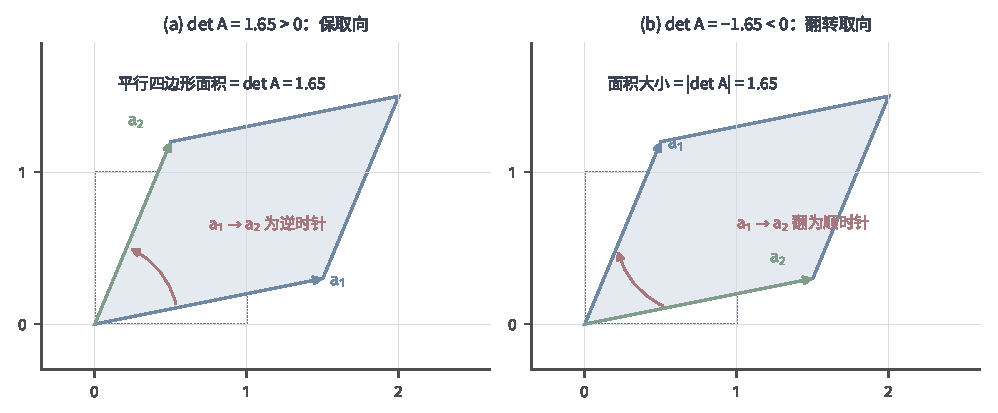
\includegraphics[width=169mm]{figures/01-mathematical-preliminaries-upper/02-linear-spaces/matplotlib/ls-determinant-oriented-volume/ls-determinant-oriented-volume.pdf}
  \caption{行列式作为有向体积的缩放。左：单位正方形由$\bm e_1=(1,0)$、$\bm e_2=(0,1)$张成，面积为$1$。中：$\bm A=\bigl(\begin{smallmatrix}2&0.5\\0&1.5\end{smallmatrix}\bigr)$把它映成由$\bm A\bm e_1=(2,0)$、$\bm A\bm e_2=(0.5,1.5)$张成的平行四边形，有向面积为$2\cdot1.5-0.5\cdot0=3=\det\bm A>0$（保定向）。右：$\bm A$把$\bm e_1$反射到$(-2,0)$，有向面积为$-3$（反定向）。向量与数值均为解析教学例。}
  \label{fig:ls-determinant-oriented-volume}
\end{figure*}

为了直接由矩阵元素计算，把$\bm A\bm e_j=\sum_i a_{i,j}\bm e_i$代入楔积展开，得到有限和
\[
 \det\bm A
 =\sum_{\pi\in S_d}\operatorname{sgn}(\pi)
   \prod_{i=1}^d a_{i,\pi(i)}.
\]
这里$S_d$是$\{1,\ldots,d\}$到自身的全部双射，每个$\pi$规定第$i$行选取第$\pi(i)$列。$d=2$时两种列次序的逆序对数分别为$0$与$1$，正好得到$ad-bc$。行列式因而是矩阵元素的多项式。例如$\begin{pmatrix}1&2\\3&4\end{pmatrix}$的行列式为$-2$，与它的迹$5$是两个不同的量。

由楔积的规则可逐条读出行列式的列变换性质：对每一列分别线性；交换两列变号，两列相同则为零；把某列的倍数加到另一列上不改变行列式。把排列展开中的$\pi$换成逆排列，得到$\det(\bm A^\top)=\det\bm A$，所以这些规则对行同样成立。三角矩阵的排列展开中只有主对角线一项非零，故三角行列式等于对角元之积，$\det\bm I_d=1$。行列式不是对整个矩阵线性的函数：$d\geq2$时一般$\det(\bm A+\bm B)\neq\det\bm A+\det\bm B$。

\paragraph{行列式乘法性与可逆判据}

复合两次作用时，体积缩放倍数应当相乘。由楔积的多线性，
\[
 (\bm A\bm B)\bm e_1\wedge\cdots\wedge(\bm A\bm B)\bm e_d
 =(\det\bm B)\,\bm A\bm e_1\wedge\cdots\wedge\bm A\bm e_d
 =(\det\bm A)(\det\bm B)\,\bm e_1\wedge\cdots\wedge\bm e_d,
\]
其中第一步把$\bm B\bm e_j=\sum_i b_{i,j}\bm e_i$代入后，$\bm A$作用在展开式的各项上，系数正是$\det\bm B$。于是
\[
 \det(\bm A\bm B)=\det\bm A\,\det\bm B.
\]
列线性相关时楔积为零，行列式为零；列线性无关时楔积非零，行列式非零。所以方阵可逆恰好等价于行列式非零，且可逆时$\det(\bm A^{-1})=1/\det\bm A$。

在第~\ref{sec:ls-matrix-equivalences}节的相似关系$\bm B=\bm P^{-1}\bm A\bm P$中，由乘法性
\[
 \det\bm B
 =\det(\bm P^{-1})\det\bm A\det\bm P
 =\det\bm A,
\]
相似变换不改变行列式；它与第~\ref{sec:ls-matrix-contractions}节迹的相似不变性一起，是判断两个矩阵能否记录同一映射时可直接计算的两个标量不变量。双线性型在两个输入同时换基时按合同$\bm B=\bm P^\top\bm A\bm P$变换，此时$\det\bm B=(\det\bm P)^2\det\bm A$：合同只保持行列式的符号与非零性，不保持数值。

\paragraph{特征多项式}

行列式把第~\ref{sec:ls-matrix-powers}节的特征值问题化为一个标量方程。$\lambda$是$\bm A$的特征值，当且仅当$(\bm A-\lambda\bm I)\bm v=\bm0$有非零解，即$\bm A-\lambda\bm I$不可逆，也即$\det(\lambda\bm I-\bm A)=0$。定义
\begin{equation}
 p_{\bm A}(z)=\det(z\bm I-\bm A),
 \label{eq:matrix-analysis-characteristic-polynomial}
\end{equation}
称为\term{特征多项式}（characteristic polynomial）。排列展开中只有对角线一项含$z^d$，故它是首项系数为$1$的$d$次实多项式，实特征值恰为它的实根。以$\bm A=\begin{pmatrix}0.8&4\\0&0.5\end{pmatrix}$为例，$p_{\bm A}(z)=(z-0.8)(z-0.5)$，与第~\ref{sec:ls-matrix-powers}节找到的两条特征方向相符；$90^\circ$旋转的特征多项式$z^2+1$没有实根，因而没有实特征向量。相似矩阵的特征多项式相同：$\det(z\bm I-\bm P^{-1}\bm A\bm P)=\det\bigl(\bm P^{-1}(z\bm I-\bm A)\bm P\bigr)=p_{\bm A}(z)$。

根$\lambda$在$p_{\bm A}$中的重数称为\term{代数重数}，特征空间的维数$\dim\ker(\bm A-\lambda\bm I)$称为\term{几何重数}。把$\lambda$的特征空间的一组基（设有$g$个向量）扩充成全空间的基，$\bm A$在新基下成为分块上三角$\begin{pmatrix}\lambda\bm I_g&*\\\bm0&\bm C\end{pmatrix}$，特征多项式含因子$(z-\lambda)^g$，故几何重数不超过代数重数。例如$\begin{pmatrix}0.8&1\\0&0.8\end{pmatrix}$的特征多项式为$(z-0.8)^2$，代数重数为$2$，几何重数却只有$1$。

不同特征值的特征空间之和是直和：若$\sum_\lambda\bm w_\lambda=\bm0$且$\bm w_\lambda$属于相应特征空间，其中非零的$\bm w_\lambda$是不同特征值的特征向量，由第~\ref{sec:ls-matrix-powers}节它们线性无关，所以每个$\bm w_\lambda=\bm0$。因此各特征空间的基合在一起仍线性无关。由此得到可对角化的判据：$\bm A$实可对角化，当且仅当$p_{\bm A}$能分解为实一次因子之积，且每个特征值的几何重数等于代数重数。充分性是因为此时几何重数之和等于$d$，各特征空间的基合成一组特征基；必要性是因为$\bm A=\bm V\bm\Lambda\bm V^{-1}$时$p_{\bm A}(z)=\prod_i(z-\lambda_i)$，$\lambda$在$\bm\Lambda$对角线上出现的次数既是代数重数，也是$\bm\Lambda-\lambda\bm I$的零空间维数，而相似变换不改变零空间维数。

\paragraph{余子式与古典伴随恒等式}

行列式还可以按一行展开。对$d\geq2$，删除第$i$行、第$j$列得到的$(d-1)$阶子矩阵记为$\bm A^{(i,j)}$，定义\term{代数余子式}（cofactor）
\[
 C_{i,j}=(-1)^{i+j}\det\bm A^{(i,j)}.
\]
把排列展开按第$i$行选取的列分类，得到$\det\bm A=\sum_{j=1}^d a_{i,j}C_{i,j}$；按列同样有$\det\bm A=\sum_{i=1}^d a_{i,j}C_{i,j}$。把全部代数余子式排成矩阵$\bm C$，其转置称为\term{古典伴随}（classical adjugate）$\operatorname{adj}(\bm A)=\bm C^\top$。

\begin{theorem}[古典伴随恒等式]
\label{thm:ls-adjugate-identity}
对任意$d$阶方阵$\bm A$，
\[
 \bm A\,\operatorname{adj}(\bm A)
 =\operatorname{adj}(\bm A)\,\bm A
 =(\det\bm A)\,\bm I_d.
\]
\end{theorem}
\begin{proof}
乘积$\bm A\bm C^\top$的$(i,k)$元素为$\sum_j a_{i,j}C_{k,j}$。当$i=k$时，这正是沿第$i$行展开的$\det\bm A$；当$i\neq k$时，它是把第$k$行换成第$i$行后的矩阵沿第$k$行的展开，新矩阵有两行相同，行列式为零。于是$\bm A\bm C^\top=(\det\bm A)\bm I_d$。按列展开同样得到$\bm C^\top\bm A=(\det\bm A)\bm I_d$。
\end{proof}

古典伴随是由余子式得到的代数构造，与第~\ref{sec:ls-adjoints}节由内积配对定义的伴随不是同一个对象。$\det\bm A\neq0$时，恒等式给出逆的代数表达$\bm A^{-1}=\operatorname{adj}(\bm A)/\det\bm A$，二阶时即$\begin{pmatrix}a&b\\c&d\end{pmatrix}^{-1}=\frac1{ad-bc}\begin{pmatrix}d&-b\\-c&a\end{pmatrix}$。高阶时展开余子式的代价是阶乘级的，恒等式主要作为证明工具，例如第~\ref{sec:ls-matrix-power-behavior}节的Cayley--Hamilton定理。

\section{张量运算}
\label{sec:ls-tensor-operations}

前面的运算大多把同类对象合成同类对象。张量运算处理多个槽位：张量积把多个输入的槽位全部保留下来，组合成一个带更多轴的对象；Kronecker积是两个矩阵的张量积在坐标下的分块记录；缩约则反过来，指定一对槽位对齐求和，把多轴对象汇总成更低阶的对象。三者共同组成多轴数据的基本运算，内积、矩阵乘法与迹都是其中的特例。

\subsection{张量积}
\label{sec:ls-tensor-products}
\label{sec:linear-algebra-joint-operations}

\subsubsection{定义与含义}

\paragraph{张量积与简单张量}

设$\bm x\in\mathbb R^m$、$\bm y\in\mathbb R^n$，它们的\term{张量积}（tensor product）$\bm x\otimes\bm y$是一个$m\times n$数组，元素为$(\bm x\otimes\bm y)_{i,j}=x_i y_j$。这样的对象称为\term{简单张量}（simple tensor）。例如$\bm x=(1,2)^\top$、$\bm y=(3,-1)^\top$给出$\bm x\otimes\bm y=\begin{pmatrix}3&-1\\6&-2\end{pmatrix}$，每一行都是$\bm y$的倍数，每一列都是$\bm x$的倍数。一般张量是若干简单张量之和$\sum_s\bm x_s\otimes\bm y_s$；并非每个二阶张量都能写成单个简单张量，正如并非每个矩阵都是秩一矩阵。图~\ref{fig:ls-tensor-product-slots} 展示张量积怎样保留两个因子的槽位。
\begin{figure}[htbp]
  \centering
  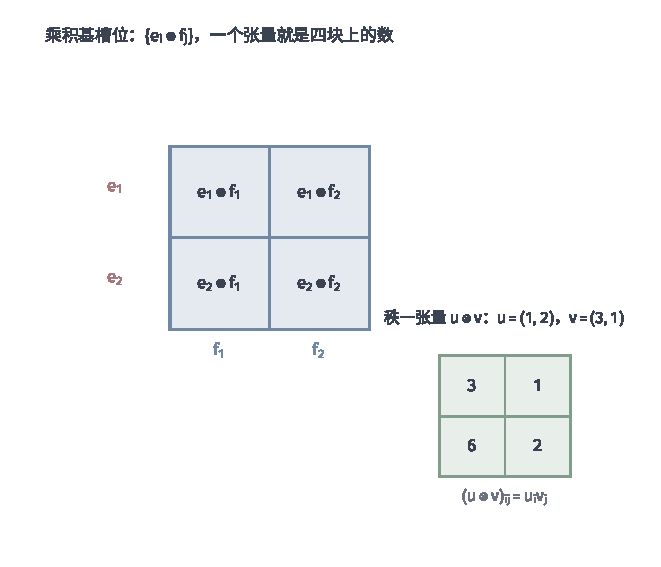
\includegraphics[width=112mm]{figures/01-mathematical-preliminaries-upper/02-linear-spaces/matplotlib/ls-tensor-product-slots/ls-tensor-product-slots.pdf}
  \caption{张量积并排保留两个因子的槽位。左：$\bm u\in\mathbb R^2$、$\bm v\in\mathbb R^3$。右：$\bm u\otimes\bm v$排成$2\times3$网格，每行由$\bm v$方向复制并按$u_i$缩放；它是秩一张量，数值由$\bm u=(1,0.6)$、$\bm v=(1,0.5,0.2)$直接相乘得到，是教学构造。}
  \label{fig:ls-tensor-product-slots}
\end{figure}

取$\mathbb R^m$的基$\bm e_i$与$\mathbb R^n$的基$\bm f_j$，产品基$\bm e_i\otimes\bm f_j$共$mn$个，构成张量积空间的一组基，故维数为$mn$。三个向量的张量积$(\bm x\otimes\bm y\otimes\bm z)_{i,j,k}=x_i y_j z_k$保留三条轴，多重张量积按同样规则逐槽位相乘。

张量积的作用是把双线性映射变成线性映射。给定双线性映射$B:\mathbb R^m\times\mathbb R^n\to W$，存在唯一的线性映射$\widetilde B:\mathbb R^m\otimes\mathbb R^n\to W$使$\widetilde B(\bm x\otimes\bm y)=B(\bm x,\bm y)$：先在产品基上规定$\widetilde B(\bm e_i\otimes\bm f_j)=B(\bm e_i,\bm f_j)$，再线性延拓即可。以欧氏内积$B(\bm x,\bm y)=\bm x^\top\bm y$为例，提升后的线性映射把$\bm x\otimes\bm y$送到$\sum_ix_iy_i$，也就是对数组$\bm x\otimes\bm y$的对角线求和——这正是后面的缩约。

二阶张量与矩阵是同一组数的两种记录：张量强调槽位来自哪一组输入，矩阵强调行列在复合中的角色。二者由第~\ref{sec:ls-reshaping}节的重排互相转换，数值不变。

\subsubsection{运算性质}

张量积对两个因子分别线性：$(a\bm x)\otimes\bm y=\bm x\otimes(a\bm y)=a(\bm x\otimes\bm y)$，且对加法分配；括号可以在槽位间移动，$(\bm x\otimes\bm y)\otimes\bm z=\bm x\otimes(\bm y\otimes\bm z)$。交换两个槽位对应轴置换：$\bm x\otimes\bm y$的$(i,j)$元素$x_iy_j$是$\bm y\otimes\bm x$的$(j,i)$元素，两者互为转置。

第~\ref{sec:ls-exterior-determinants}节的楔积可以由张量积经反对称化得到：$\bm x\wedge\bm y$对应$\bm x\otimes\bm y-\bm y\otimes\bm x$。这里只指出联系，楔积的构造不依赖张量积。

在Frobenius内积下，简单张量的配对与范数都分离：
\[
 \langle\bm x\otimes\bm y,\bm x'\otimes\bm y'\rangle_{\mathrm F}
 =\langle\bm x,\bm x'\rangle\langle\bm y,\bm y'\rangle,
 \qquad
 \lVert\bm x\otimes\bm y\rVert_{\mathrm F}=\lVert\bm x\rVert\,\lVert\bm y\rVert,
\]
因为$\sum_{i,j}x_iy_jx'_iy'_j=(\sum_ix_ix'_i)(\sum_jy_jy'_j)$。以$\bm x=(1,2)^\top$、$\bm y=(3,-1)^\top$为例，乘积范数为$\sqrt5\cdot\sqrt{10}=5\sqrt2$，与直接对$\begin{pmatrix}3&-1\\6&-2\end{pmatrix}$求Frobenius范数一致。

\paragraph{Schur乘积定理}

配对的分离性给出一个关于逐项乘积的结论。设$\bm A,\bm B$均为半正定矩阵，由定理~\ref{thm:ls-gram-factor}，它们各有Gram因子$\bm A=\bm U^\top\bm U$、$\bm B=\bm V^\top\bm V$，即$A_{i,k}=\langle\bm u_i,\bm u_k\rangle$、$B_{i,k}=\langle\bm v_i,\bm v_k\rangle$，其中$\bm u_i,\bm v_i$是两个因子的列。考虑向量组$\{\bm u_i\otimes\bm v_i\}$，其Gram矩阵为
\[
 \langle\bm u_i\otimes\bm v_i,\bm u_k\otimes\bm v_k\rangle_{\mathrm F}
 =\langle\bm u_i,\bm u_k\rangle\langle\bm v_i,\bm v_k\rangle
 =A_{i,k}B_{i,k}.
\]
Gram矩阵恒半正定，故逐项乘积$\bm A\odot\bm B$半正定，这就是\term{Schur乘积}定理。例如$\bm A=\bm B=\begin{pmatrix}1&1\\1&2\end{pmatrix}$，逐项乘积$\begin{pmatrix}1&1\\1&4\end{pmatrix}$的行列式为$3>0$、对角元为正，仍半正定。核方法中两个核矩阵的逐项乘积仍是合法核矩阵，依据就是这一定理。

\subsection{Kronecker积}
\label{sec:ls-kronecker-products}

当两个因子本身都是矩阵时，张量积空间上的联合作用可以写成一张分块矩阵，这就是Kronecker积。

\subsubsection{定义与含义}

\paragraph{Kronecker积的定义}

对$\bm A\in\mathbb R^{m\times n}$、$\bm B\in\mathbb R^{p\times q}$，定义
\begin{equation}
 \bm A\otimes\bm B
 =\begin{bmatrix}
  A_{1,1}\bm B&\cdots&A_{1,n}\bm B\\
  \vdots&\ddots&\vdots\\
  A_{m,1}\bm B&\cdots&A_{m,n}\bm B
 \end{bmatrix}\in\mathbb R^{mp\times nq}.
 \label{eq:linear-algebra-kronecker-product}
\end{equation}
每个块$A_{i,j}\bm B$是$\bm B$整体乘以$A_{i,j}$。图~\ref{fig:ls-kronecker-block-structure} 展示这种逐元素替换的分块结构。
\begin{figure}[htbp]
  \centering
  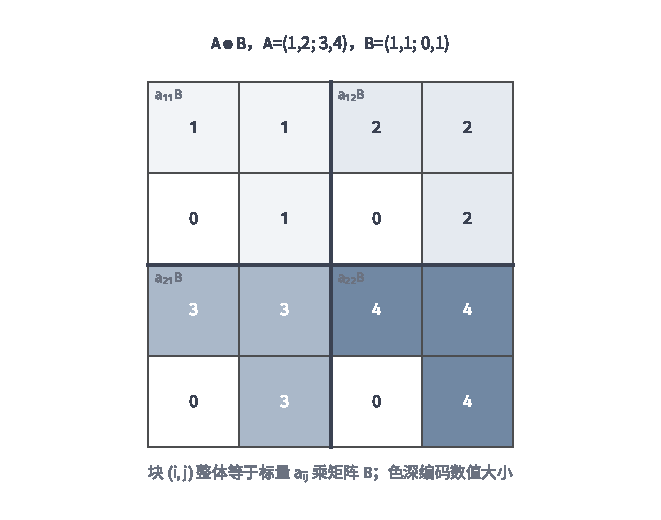
\includegraphics[width=112mm]{figures/01-mathematical-preliminaries-upper/02-linear-spaces/matplotlib/ls-kronecker-block-structure/ls-kronecker-block-structure.pdf}
  \caption{Kronecker积的分块结构。上：$\bm A=\bigl(\begin{smallmatrix}1&2\\3&4\end{smallmatrix}\bigr)$、$\bm B=\bigl(\begin{smallmatrix}10&20\\30&40\end{smallmatrix}\bigr)$。下：$\bm A\otimes\bm B$是把$\bm A$的每个元素替换为该元素乘$\bm B$得到的$4\times4$分块矩阵，块边界用白线强调。数值由定义直接计算，是教学例。}
  \label{fig:ls-kronecker-block-structure}
\end{figure}

在产品基$\bm e_i\otimes\bm f_j$下，$(\bm A\otimes\bm B)(\bm x\otimes\bm y)=(\bm A\bm x)\otimes(\bm B\bm y)$：第一个槽位只经过$\bm A$，第二个槽位只经过$\bm B$，两个作用并行而不串联。这与矩阵乘法把前后两次作用串成一条链形成对照。向量的张量积是它的特例：两个列向量的Kronecker积就是按行展开的$\bm x\otimes\bm y$。

\subsubsection{运算性质}

按成对索引分别求和，相容乘积满足混合乘积规则
\begin{equation}
 (\bm A\otimes\bm B)(\bm C\otimes\bm D)
 =(\bm A\bm C)\otimes(\bm B\bm D),
 \label{eq:matrix-analysis-kronecker-mixed-product}
\end{equation}
其中$\bm A\bm C$与$\bm B\bm D$分别相容：左侧的块$(i,k)$为$\sum_jA_{i,j}C_{j,k}\bm B\bm D$，恰是右侧的块。由此得到$(\bm A\otimes\bm B)^\top=\bm A^\top\otimes\bm B^\top$；两因子都可逆时$(\bm A\otimes\bm B)^{-1}=\bm A^{-1}\otimes\bm B^{-1}$；方阵情形下$\operatorname{tr}(\bm A\otimes\bm B)=\operatorname{tr}\bm A\operatorname{tr}\bm B$。

结合第~\ref{sec:ls-reshaping}节的向量化，对$\bm A\in\mathbb R^{p\times m}$、$\bm X\in\mathbb R^{m\times n}$、$\bm B\in\mathbb R^{n\times q}$，
\begin{equation}
 \operatorname{vec}(\bm A\bm X\bm B)
 =(\bm B^\top\otimes\bm A)\operatorname{vec}(\bm X).
 \label{eq:matrix-analysis-vec-kronecker}
\end{equation}
证明只需比较输出元素：两侧的$(i,j)$元素均为$\sum_{\ell=1}^m\sum_{k=1}^n A_{i,\ell}X_{\ell,k}B_{k,j}$。固定$\bm A,\bm B$后这是关于$\bm X$的线性映射，把两侧同时作用于未知矩阵的方程化成普通线性方程组。

表~\ref{tab:linear-algebra-products-and-shapes}汇总本章几种“乘法”的形状条件与索引作用。

\begin{table*}[htbp]
 \centering\small
 \begin{tabularx}{\linewidth}{@{}lXX@{}}
  \toprule
  运算 & 形状条件与输出 & 索引作用\\
  \midrule
  $\bm A\bm B$ & $(m\times n)(n\times p)\to m\times p$ & 汇总共同索引\\
  $\bm A\odot\bm B$ & 同为$m\times n$，输出仍为$m\times n$ & 同位置相乘，不求和\\
  $\bm A\otimes\bm B$ & $(m\times n)$与$(p\times q)\to(mp)\times(nq)$ & 保留两组成对索引\\
  $\langle\bm x,\bm y\rangle$ & 两个$n$维向量，输出标量 & 配对后汇总\\
  \bottomrule
 \end{tabularx}
 \caption{相乘符号对应不同操作。先检查消去哪些索引，再判断其线性性和输出含义。}
 \label{tab:linear-algebra-products-and-shapes}
\end{table*}

\subsection{张量缩约}
\label{sec:ls-tensor-contraction}

张量积把槽位全部保留，缩约则指定一对相容槽位，对齐相乘后求和，消去这对轴。

\subsubsection{定义与性质}

\paragraph{张量缩约的定义}

缩约须先指定参与求和的轴，并保证对应尺寸相同。例如$\bm A\in\mathbb R^{m\times d\times r}$、$\bm B\in\mathbb R^{d\times n\times r}$可定义
\[
 c_{i,j}=\sum_{k=1}^d\sum_{s=1}^r a_{i,k,s}b_{k,j,s},
\]
同时消去$k$与$s$两对轴。被求和的轴消失，其余轴保留：上例输出为$m\times n$矩阵。矩阵乘法是只消去一对轴的特例，内积是两个向量唯一一对轴的缩约。对$\bm X\in\mathbb R^{b\times\ell\times d}$的最后一轴作用$\bm W\in\mathbb R^{d\times h}$，$z_{i,j,r}=\sum_k x_{i,j,k}w_{k,r}$，输出形状为$b\times\ell\times h$。写出索引就能检查哪些轴被消去、哪些轴应当保留。图~\ref{fig:ls-tensor-contraction} 沿一对选中的轴求和并保留其余轴。
\begin{figure}[htbp]
  \centering
  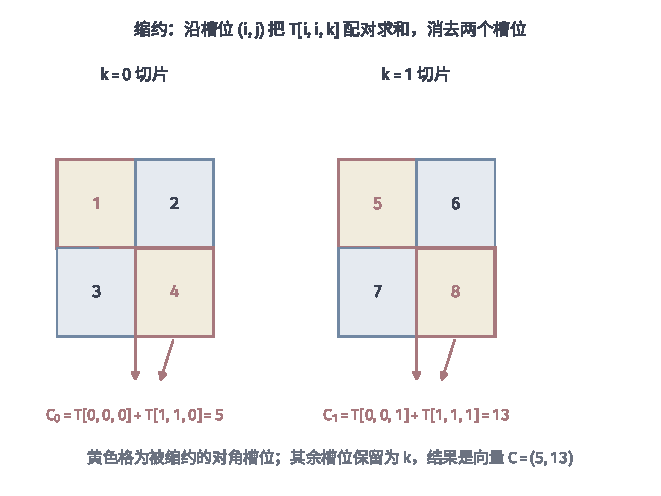
\includegraphics[width=112mm]{figures/01-mathematical-preliminaries-upper/02-linear-spaces/matplotlib/ls-tensor-contraction/ls-tensor-contraction.pdf}
  \caption{张量缩约沿选中的一对轴求和、保留其余轴。左：二阶张量按行和列着色；选中列轴（虚线箭头）沿列求和，输出对每行汇总为一个值。右：缩约后得到$3$个输出，分别对应原矩阵三行的行和，颜色由红(小)经黄到蓝(大)。张量与数值均为解析教学例。}
  \label{fig:ls-tensor-contraction}
\end{figure}

系数是简单张量时，缩约可以分开计算。一次读取同时依赖三组向量$\bm x\in\mathbb R^m$、$\bm y\in\mathbb R^n$、$\bm z\in\mathbb R^p$时，若系数数组是秩一张量$\bm a\otimes\bm b\otimes\bm c$，则
\begin{equation}
 \left\langle\bm a\otimes\bm b\otimes\bm c,
 \bm x\otimes\bm y\otimes\bm z\right\rangle_{\mathrm F}
 =(\bm a^\top\bm x)(\bm b^\top\bm y)(\bm c^\top\bm z),
 \label{eq:linear-algebra-rank-one-contraction}
\end{equation}
三重求和分离成三个内积的乘积。例如取$\bm a=(1,2)^\top$、$\bm b=(3,-1)^\top$、$\bm c=(2,1)^\top$，$\bm x=(2,1)^\top$、$\bm y=(1,1)^\top$、$\bm z=(1,-1)^\top$，三个内积依次为$4,2,1$，读取等于$8$。

固定配对对象后，缩约对被作用张量线性。多对轴的缩约是有限和，求和次序可以交换，结果与先消哪一对轴无关。$\operatorname{softmax}$、逐元素非线性等操作不属于缩约：一个模型即使由缩约和这些操作交替组成，固定系数时的线性也不代表整体线性。

\subsubsection{矩阵上的缩约}
\label{sec:ls-matrix-contractions}
\label{sec:prelim-matrix-trace}

\paragraph{迹的定义}

方阵最自然的缩约是把行轴与列轴对齐到同一索引后求和。对$n$阶方阵，定义\term{迹}（trace）
\[
 \operatorname{tr}(\bm A)=\sum_{i=1}^n A_{i,i}.
\]
例如$\bm A=\begin{pmatrix}1&2\\3&4\end{pmatrix}$的迹为$1+4=5$。迹是对角元之和，不是全部元素之和。有限和的线性规则直接给出$\operatorname{tr}(a\bm A+b\bm B)=a\operatorname{tr}(\bm A)+b\operatorname{tr}(\bm B)$。

矩阵乘法没有交换律，但乘积的迹在合法的循环移位下不变。对$\bm A\in\mathbb R^{m\times n}$、$\bm B\in\mathbb R^{n\times m}$，有限和换序给出
\begin{equation}
 \operatorname{tr}(\bm A\bm B)
 =\sum_{i=1}^m\sum_{j=1}^n A_{i,j}B_{j,i}
 =\operatorname{tr}(\bm B\bm A).
 \label{eq:linear-algebra-trace-cyclic}
\end{equation}
两个乘积甚至可以是不同阶的方阵；相等的是迹，不是矩阵本身。三因子只能循环移动，$\operatorname{tr}(\bm A\bm B\bm C)=\operatorname{tr}(\bm B\bm C\bm A)=\operatorname{tr}(\bm C\bm A\bm B)$，不能任意交换相邻因子：取$\bm A=\begin{pmatrix}1&0\\0&0\end{pmatrix}$、$\bm B=\begin{pmatrix}0&0\\1&0\end{pmatrix}$、$\bm C=\begin{pmatrix}0&1\\0&0\end{pmatrix}$，则$\bm A\bm B\bm C=\bm0$，而$\bm A\bm C\bm B=\begin{pmatrix}1&0\\0&0\end{pmatrix}$，迹分别为$0$与$1$。由循环性，相似变换不改变迹：
\[
 \operatorname{tr}(\bm P^{-1}\bm A\bm P)
 =\operatorname{tr}(\bm A\bm P\bm P^{-1})
 =\operatorname{tr}\bm A.
\]
迹与行列式一样，是第~\ref{sec:ls-matrix-equivalences}节相似关系下的标量不变量。

第~\ref{sec:ls-inner-products}节定义的Frobenius内积把对应位置相乘后相加，写成缩约就是
\[
 \langle\bm A,\bm B\rangle_{\mathrm F}
 =\sum_{i,j}A_{i,j}B_{i,j}
 =\operatorname{tr}(\bm A^\top\bm B),
\]
因为$\bm A^\top\bm B$第$j$个对角元为$\sum_i A_{i,j}B_{i,j}$，再对$j$求和恰好遍历所有位置。计算$\operatorname{tr}(\bm A\bm B)$时也不必形成乘积：只需$\sum_{i,j}A_{i,j}B_{j,i}$，代价为$mn$而非$m^2n$。

\section{本章小结}
\label{sec:ls-operations-summary}

本章回答第~\ref{chap:linear-representation}章记录下来的对象怎样运算。对每种运算，我们都规定了输入的相容条件与输出形状，说明了它的运算逻辑，并给出可以直接使用的性质。

第一组运算把对象合并成同类对象。加法与数乘要求形状一致，线性组合把多个记录合成一个，映射的叠加对应矩阵的逐项相加。“乘法”有两种含义：逐项乘法在同一位置相乘、不汇总任何索引，依赖坐标；矩阵乘法来自映射复合，汇总共同索引，满足结合律而不满足交换律。分块后块可以像数一样相乘。同一方阵的反复作用得到矩阵幂；特征方向是幂在其上只作标量缩放的方向，可对角化时幂化为对角元的乘方。转置、轴置换、reshape与向量化只改变记录位置，不改变数值，但会改变秩与诱导范数这类依赖排列的量。

第二组运算给对象以几何。内积把两个对象配成标量，由Cauchy--Schwarz不等式得到夹角；加权内积由正定矩阵给出，Gram因子定理说明它只是换了一组欧氏坐标；Gram矩阵记录一组向量的全部配对，非奇异当且仅当它们线性无关，由此得到正交直和。范数给出误差的大小：$\ell_p$范数由Hölder不等式联系，诱导矩阵范数度量最坏放大并满足次乘性，对偶范数回答线性读取在误差预算下的最大变化。伴随把内积配对中的作用从输出端搬到输入端，标准内积下就是转置，加权内积下要带上两侧权重。

第三组运算处理多个槽位。外积用交替多线性记录有向体积，最高维系数就是行列式：它满足乘法性，非零当且仅当矩阵可逆，并把特征值问题化为特征多项式的求根；几何重数与代数重数是否相等决定能否对角化。张量积保留全部槽位，Kronecker积是矩阵张量积的分块记录，混合乘积规则与向量化恒等式把两者与普通矩阵乘法联系起来；缩约沿指定槽位求和，矩阵乘法、内积与迹都是它的实例。

这些运算都在精确输入、一次计算的前提下讨论。点到子空间的最近点、方程的求解与逼近在第~\ref{chap:linear-equations-and-optimization}章展开，有限维范数之间的比较也在那里随距离问题建立；矩阵指数等矩阵函数、输入误差的放大与反复作用的长期行为留给第~\ref{chap:linear-analysis}章。

